\chapter{Augmediated reality system based on 3D camera self-gesture sensing}
\label{ar3dgesture}

% As a general rule, do not put math, special symbols or citations
% in the abstract
%\section{Abstract}
Three Dimensional (3D) range cameras have recently appeared in the marketplace for use in surveillance
(e.g. cameras affixed to inanimate objects) applications. In this chapter, FreeGlass as a wearable hands-free 3D gesture-sensing Digital Eye Glass system is presented. FreeGlass comprises a head-mounted display with an infrared range camera, both connected to a wearable computer and Digital Eye Glass system which embodies HDR (High Dynamic Range) and AR (Augmented/Augmediated Reality). FreeGlass recontextualizes the 3D range camera as a sousveillance (e.g. cameras attached to people) camera. In this sousveillance context, the range camera is worn by the user and shares the same point-of-view as the user. Computer vision algorithms therefore benefit from the use of the range camera to allow image segmentation by using both the infrared and depth information from the device for 3D hand gesture recognition system. The gesture recognition is then accomplished by using a neural network on the segmented hand. Recognized gestures are used to provide the user with interactions in an augmediated reality environment. Additionally, we present applications of FreeGlass for serendipitous gesture recognition in everyday life, as well as for interaction with real-world objects (with and without gesture recognition)~\cite{buchmann2004fingartips,billinghurst2001collaboration,billinghurst2008tangible,kawashima2001magic}. A plurality of FreeGlass units can be used together, each sensor having a different spreading sequence, or the like, so that a number of people can collaborate and share the same or similar Augmediated Reality space(s)~\cite{billinghurst2002collaborative,billinghurst2000mixing}.

\begin{figure}
\begin{subfigure}[b]{\columnwidth}
\centering
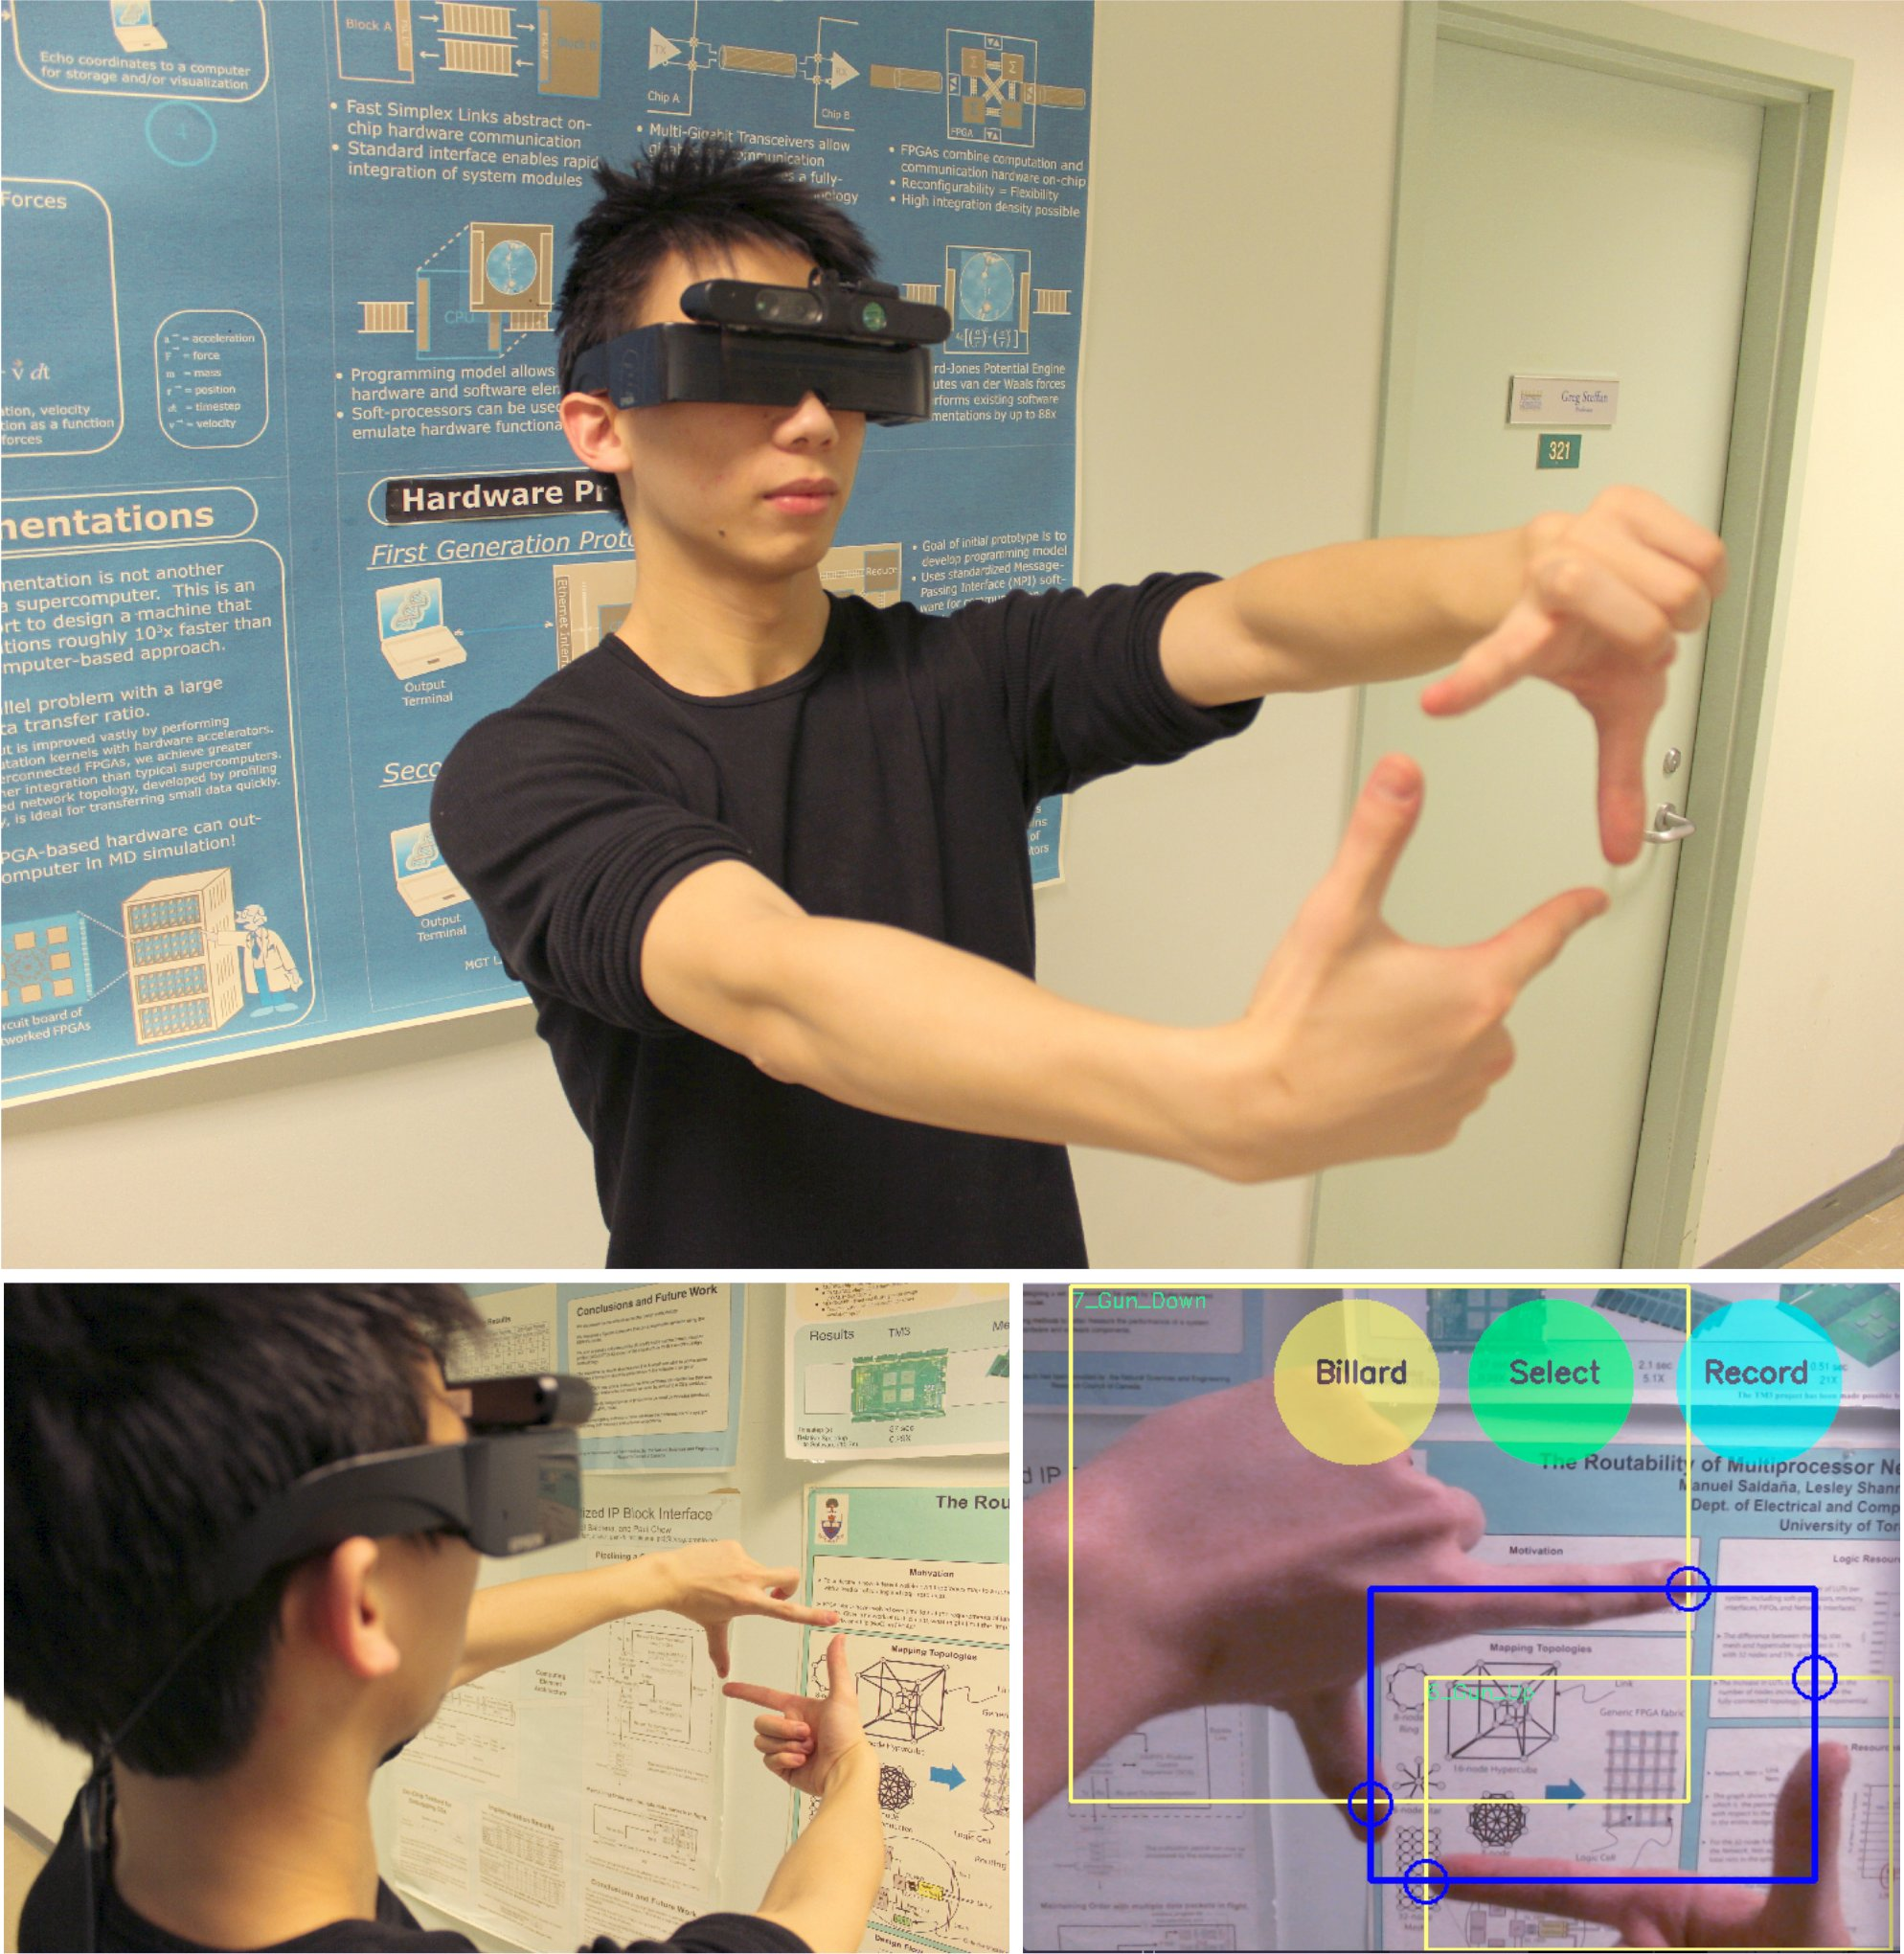
\includegraphics[width=0.6\columnwidth]{ch5/figs/crop_sample.jpg}
\end{subfigure}
\begin{subfigure}[b]{\columnwidth}
\centering
\vspace{.032in}
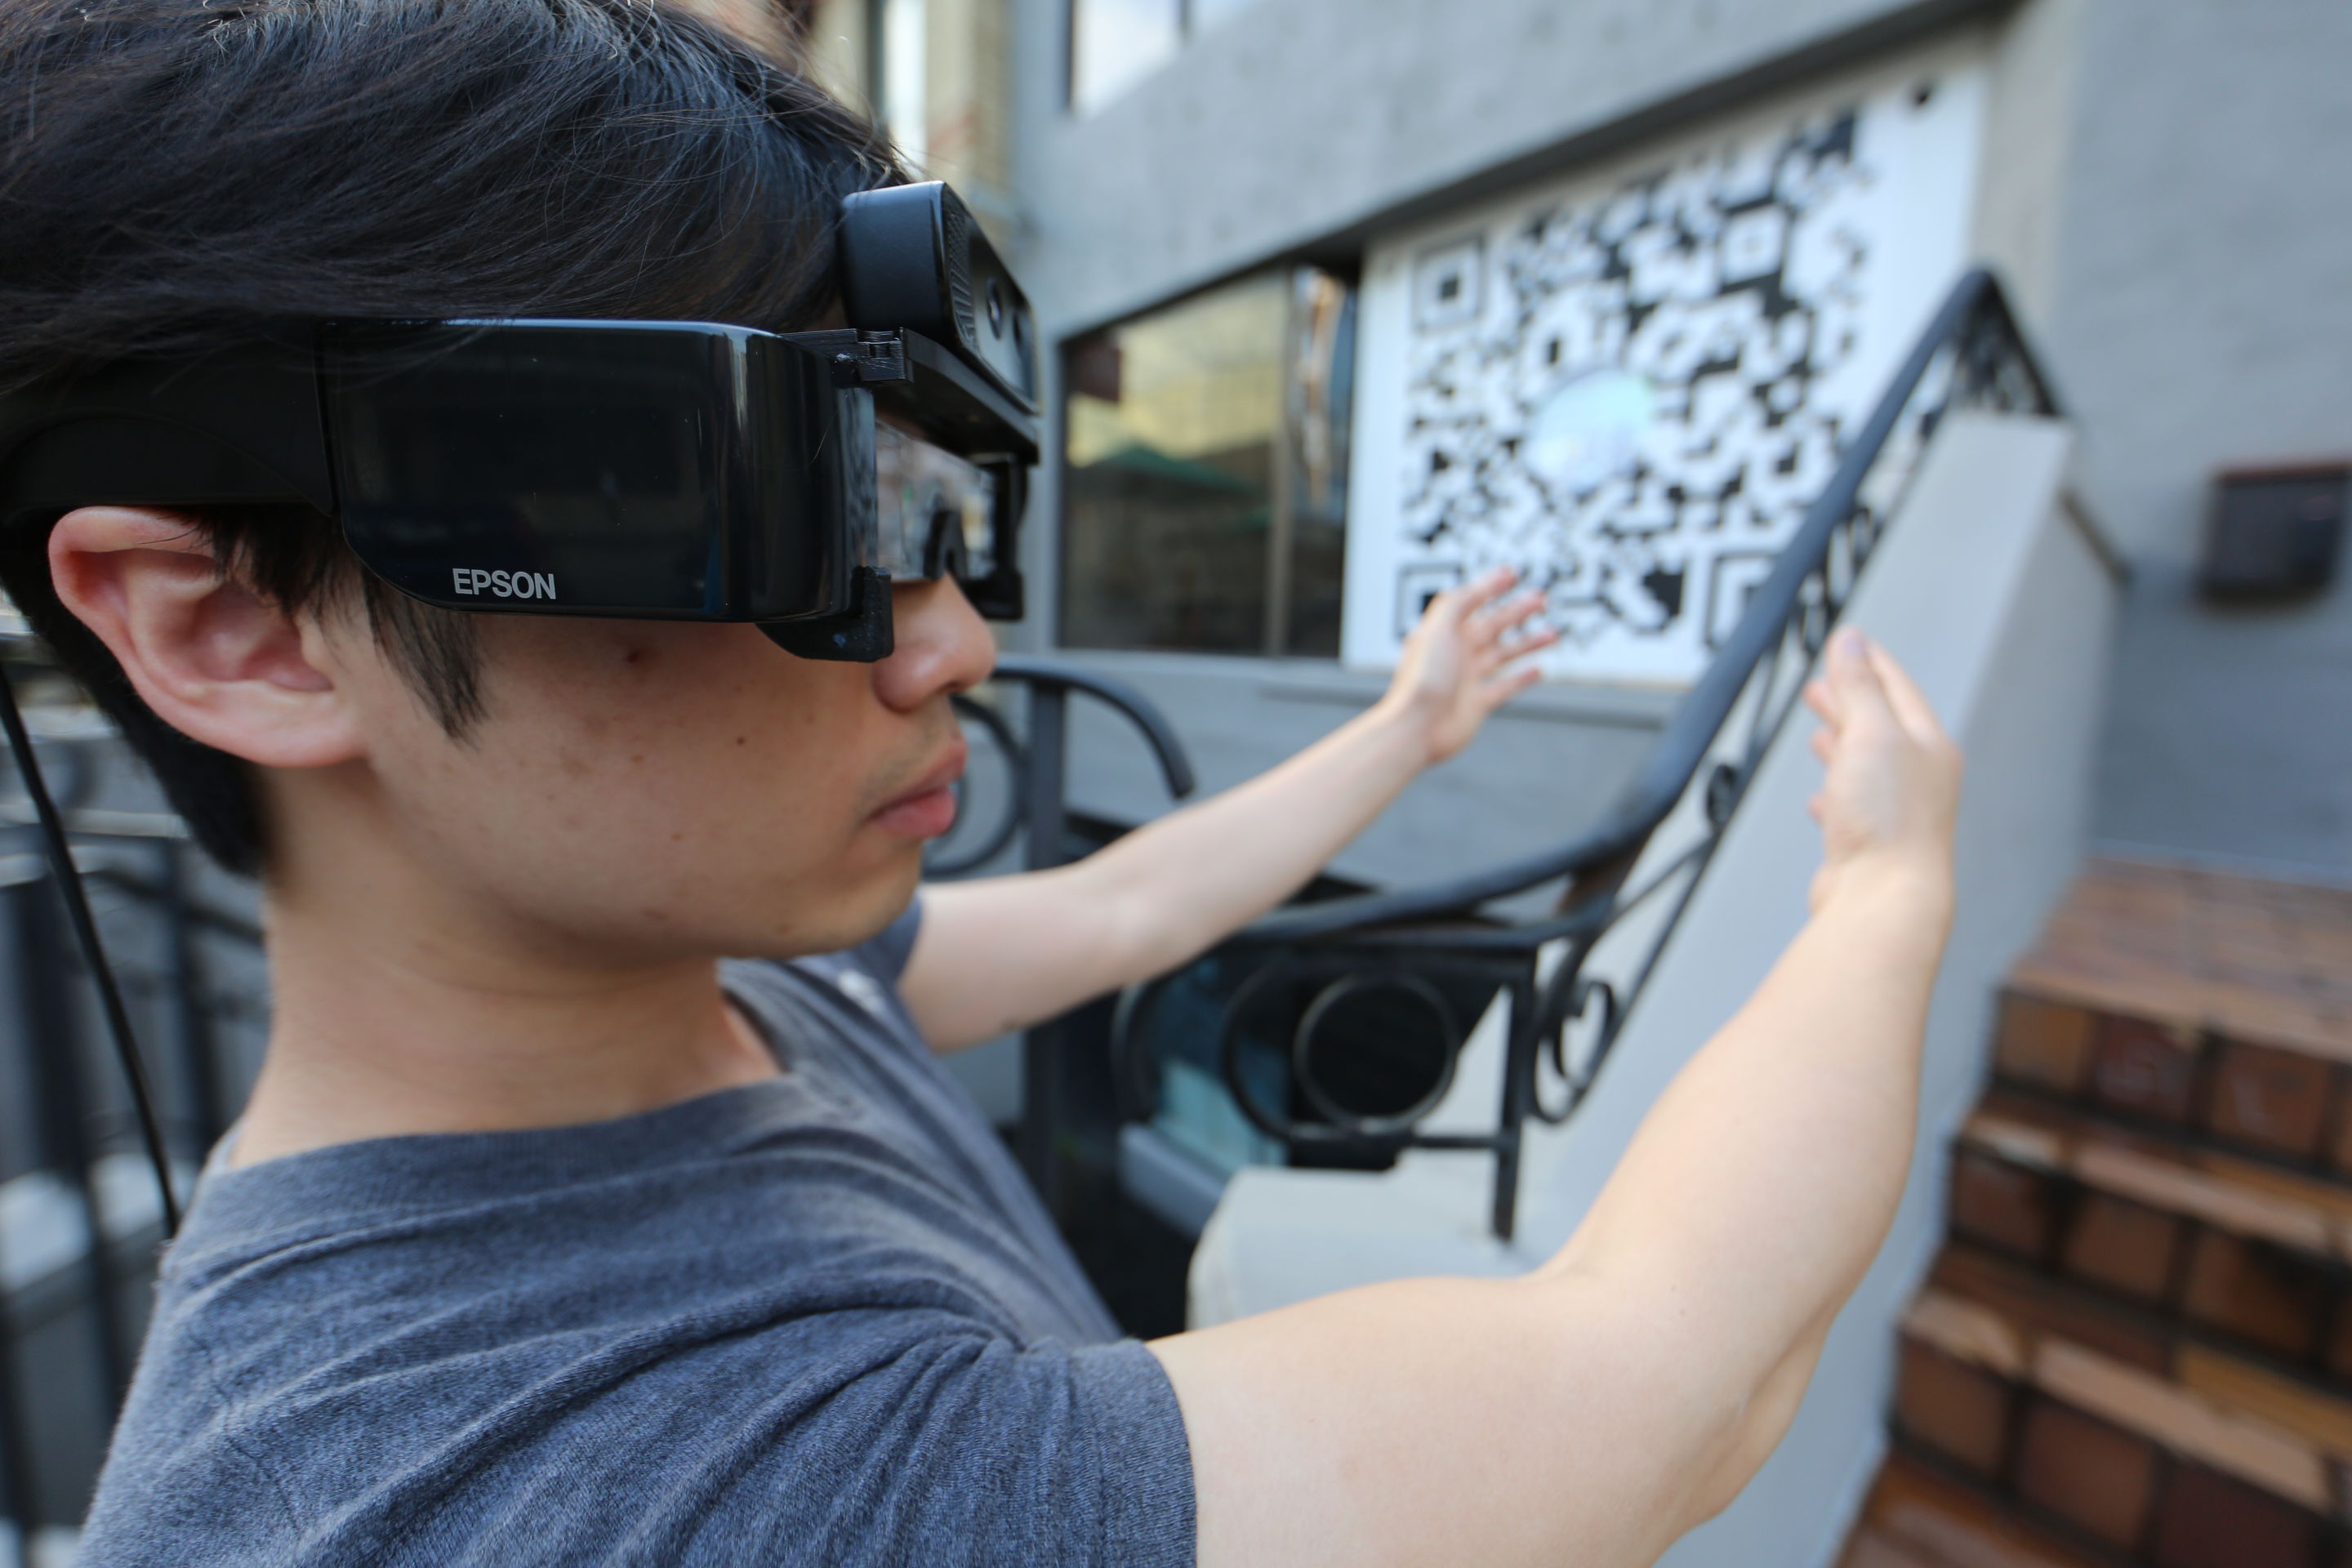
\includegraphics[width=0.6\columnwidth]{ch5/figs/wearable/low_res/qr_eyeglass_IMG_2092.jpg}
\end{subfigure}
\caption{In one practical embodiment, FreeGlass comprises a range sensing camera such
as the ASUS Xtion 3D sensor, or a Time-of-Flight (TOF) 3D sensing camera,
and a head-worn display such as the Epson Moverio BT-100 (head-mounted display),
both connected to a wearable computer such as the
ODROID-X2 ``mobile computer''.
The resulting system provides for self gesture-sensing
augmediated reality applications.
By ``self gesture'' we mean a gesture to one's self, i.e. as sensed by
a wearable camera system.
The range camera is mounted onto the wearable display and views the world from
the user's point of view, aligning with the displayed subject matter.}
\end{figure}

%\section{Introduction}
\section{Introduction}
In recent years, gesture-based controls have been incorporated into various
mobile devices such as smartphones and tablets~\cite{androidgestures,bbgeestures,bbgesturesz10}. Most of these
devices rely on the multi-touch surface as their gesture interfaces. Other
gesture recognition systems, such as the Microsoft Kinect, utilize an
infrared range camera as the input device~\cite{msprimesense2010press},
which provides the user with ``hands-free'' input (not needing to hold any
devices), via gestures. However, these devices, whether they require physical
interaction or not, are usually external to the user. The user interacts
with the device from a third person perspective. For example, consider
the Microsoft Xbox Kinect. It functions as a
surveillance camera, i.e. as part of the user's environment
rather than as part of the user (sousveillance). Both the user and
the Kinect can be considered separate entities in
this interaction - once the user walks away from the Kinect, or because
the Kinect is not always on and always with the user,
there is no constancy of interaction.
Essentially, these devices we use in some aspects of our everyday lives
are not integrated with us for use in all aspects of our lives.

The principle of Humanistic Intelligence (HI)~\cite{mann2001wearable}
and Natural User Interfaces~\cite{mann2001intelligent}
can be used to overcome this separation of user and device. That is,
by using a wearable computer, there need not be a separation of device and
the user --- the user can be part of the computational
feedback loop to the device.

The proposed 
``(hands)FreeGlass'' is a hands-free
DEG (Digital Eye Glass) input/output device that is always ready
to accept input of the user, regardless of time or
space~\cite{mann1998wearcam, mann1997wearable, mannaaai361, mistry2009sixthsense}.
The term ``digital eye glass'' and ``digital welding glass''  had been discussed over the past 20 years or so,
but it did not start to appear in the mainstream until about 10 years ago~\cite{Deg}.
FreeGlass is a DEG that combines an HI wearable system with an infrared range camera, allowing the user to
gain ``hands-free'' natural interaction that can include the use of gestures.
The term ``FreeGlass'' suggests freedom and transparency on various practical, social, technological, and philosophical levels. By ``Free'', we mean the word in the Richard Stallman sense,
i.e. ``free as in free speech'' and ``free as in free beer''.
The design is simple enough that others can freely replicate it, from widely available low-cost
commercial off-the-shelf products (displays, range cameras, and small mobile computers that can be easily re-purposed to being wearable computers).
The concept of being freely (widely) available, also connects with ideas of freedom
to tinker (freedom-to-tinker.com), ``Tinquiry'' (tinkering as a form of inquiry),
Maktivism (making as a form of social inquiry), and ``Haccessibility''
(ability to re-purpose, redesign, etc., devices for improved
accessibility, as well as making technologies to help provide accessibility,
e.g. DEG as a seeing aid).
FreeGlass also embodies aspects of reciprocal transparency,
i.e. ``veillance'' (watching) rather than only the one-sided
``surveillance'' (watching from above).
And of course the interactions can be ``hands-{\bf free}''.

\subsection{Augmediated Reality}
FreeGlass can also help people see/sense their environments better,
through Augmediated Reality. Augmediated is a portmanteau of augmented and mediated, referring to an ability not merely to add overlays (augment) but also to subtract (e.g. deliberately diminish) or modify. Examples include the work described in previous chapter that diminishes the bright light of an electric welding arc and simultaneously augments the darker areas of the scene, in addition to providing computerized overlays to annotate a
workpiece being welded~\cite{lo2012high,mann2012hdrchitecture,mann2012realtime}. Furthermore,
the ability to sense and process depth information via the Digital Eye Glass can even be beneficial to people who have vision impairments. For example, we can turn the FreeGlass into a navigation tool for the visually impaired~\cite{mann2011blind}. 

Specifically an Augmediated Reality device is a device comprising the following three elements:
\begin{itemize}
 \item an image sensor, e.g. camera, image sensor array with appropriate optics,
       or the like;
 \item an image processor responsive to an output of said image sensor;
 \item a display responsive to an output of said image processor.
\end{itemize}

\begin{figure*}
\centering

\includegraphics[width=\columnwidth]{ch5/figs/train_flow3.pdf}
\caption{The masked images are cropped, down sampled, and then processed through the neural net to determine the gesture.}
\label{flow_diagram}
\end{figure*}

\section{3D Hand Gesture Recognition}
Hand gesture recognition consists of two main components:
\begin{enumerate}
    \item Hand detection
    \item Gesture recognition.
\end{enumerate}
Hand detection concerns itself with how to robustly determine the contour of the hand in an environment with a complex background. Gesture recognition concerns itself with correctly interpreting each gesture.

To achieve hand detection, many researchers take advantage of controlled environments, such as those having constant lighting and a static background, e.g. no relative motion between the camera and the
background~\cite{imagawa1998color, hong2000gesture}. However, these methods are not reliable in the real world in uncontrolled everyday moving environments with complex lighting and continuous
background changes. Particularly, our proposed system utilizes a wearable camera that is always moving relative to the background, and thus the assumption of having a static background is often not applicable. Other methods focus on tonal based features, such as skin color segmentation~\cite{kjeldsen1996toward}. These features are not robust against dynamic lighting condition and non-static backgrounds, for example, similar colours between the background and human skin. In addition, some methods use specially coloured gloves or other sensing device such as the data glove to provide additional information for the segmentation~\cite{sturman1994survey}.
Recognizing the problems in the methods discussed above, we explore an alternative method based on the depth information provided by an infrared range camera, such as a PrimeSense camera, to perform close range hand
detection, segmentation, etc., as well as discernment between foreground (one's own hands) and background.

Whereas surveillance-based systems can use background subtraction, and thus can actually work quite well even with 2D cameras, the newer 3D cameras actually provide much greater benefit to wearable applications than they do to their original surveillance (cameras affixed in the environment) applications.

The PrimeSense 3D camera computes a depth map which contains information of an object's distance with respect to the camera. The depth map can be considered as an additional dimension of information for feature extraction
and image segmentation~\cite{ren2011robust, uebersax2011real}.

Most of the current approaches use infrared range cameras only from a third person
perspective (i.e. surveillance). In these third-person applications the assumption is made that there is no confusion between the hand's depth information with other objects in the environment. Besides the infrared range camera, some approaches use a combination of a single color camera, a stereo color camera and a thermal camera to obtain additional information for image processing and image de-noising~\cite{appenrodt2010data}. These methods achieve promising results in the static indoor setting for which they were designed.

Other gesture recognition devices such as the Leap Motion controller are
designed to capture hand gestures from a bottom-up perspective~\cite{leapmotion}. Only more recently, a head-mounted setup of Leap Motion controller was released and provided robust hand tracking with pose estimation. Since this device is not equipped with a color camera, it is not the ideal candidate for wearable augmented/mediated/augmediated reality applications where the gesture command needs to be recognized in the real world of everyday life outside the confines of a controlled environment. Also, there are software
solutions capable of recognition, such as OpenNI. OpenNI consists of a set of
open source APIs that allow us to capture natural interaction between human
and computer via PrimeSense cameras~\cite{openniabout}. Algorithms such as
skeleton tracking can effectively track the human body and its parts
by utilizing depth map information~\cite{primesensenite2}. However,
the application's gesture commands are performed in a very close range setting since the camera
is mounted on the user's head. For this reason, in self-gesturing, the gesture commands are not
recognizable by the depth map algorithms provided by the OpenNI framework.

Lastly, other 3D cameras such as the true time-of-flight camera
from SoftKinetic\footnote{http://www.softkinetic.com/fr-be/products/depthsensecameras.aspx} can
be used to perform the segmentation and extraction of hand features with our
FreeGlass system (see Figure~\ref{fig:3Dcamera_head}). However, these
sensors are designed for short range depth extraction and thus lack the ability
to sense the environment for augmediated reality purposes. The current
limitations and the future direction of a novel hybrid sensor approach will
be further discussed in the future work section.

\subsection{Proposed Method}
For a mobile or a wearable platform, we attempt to minimize the number of
devices in the system and instead of performing gesture recognition
using a 3D camera from a third-person view, where the camera observes the
user's gestures on a steady platform~\cite{li2009real}, we propose to use
the camera from the first-person perspective, where it is mounted on the
user's eye glass and observes the world from the user's point of
view~\cite{mann2011blind}. Therefore, a wearable construct based on
a 3D camera is of interest, which has appeared in the use of the navigation
helmet proposed by Mann et. al~\cite{mann2011blind}.

Similar to methods \cite{li2009real, kjeldsen1996toward, ren2011robust, uebersax2011real},
we achieve our gesture recognition in two stages:
\begin{enumerate}
\item segmentation
\item classification
\end{enumerate}

The purpose of the segmentation stage is to first locate the hands of the user in the image. We apply the classification algorithm to the segmented image to identify the gesture.

\subsection{Segmentation}
In order for the system to classify the gesture, it needs to first identify the regions which contain the user's hand(s). With our unique configuration,
we can assume the hands appear as objects within close proximity to the camera.
This information can be obtained from the range camera sensor,
like a PrimeSense or other similar camera. These cameras provides two
types of images:
\begin{enumerate}
\item Infrared image
\item Computed depth map
\end{enumerate}
The infrared image is a greyscale image that shows the level of infrared
light sensed by the camera. The depth map is provided by the camera which
approximates the distance to the objects in the scene. The two images are
filtered independently to remove ``noise'' (outliers),
i.e. pixels that do not meet certain
constraints/thresholds. The results are two binary images that intersect
to produce the final image mask, a binary image for hand extraction as
shown in Figure~\ref{image_segmentation}.

In our first simple embodiments, due to device limitations, the depth map
can only return a finite range of distance values. This is a known hardware
specification in the long range sensors where the IR laser projector
overpowers (i.e., overexpose) the subjects that are close range. A depth map
pixel is set to zero if the viewing object is either too close or too far from
the camera. Additionally, the distance of any light source or reflective
material in the scene that corrupts the projected pattern is unknown and set
to zero. With the camera worn on the user's head, we assume that the gestures
appear within the distance range up to one's fully stretched arm length away
from the head worn camera. This means that objects with depth values under
certain threshold $d_{th}$ are considered as candidates for the user's hand(s).
However, this includes false candidates such as light sources, shadows,
reflective objects, and distant objects mistakenly classified as close.
The resulting binary image sets the pixels under $d_{th}$ to one and others
are set to zero.

Since the PrimeSense camera projects the patterns in the infrared spectrum,
given the condition that no other infrared light source is present,
the objects closer to the camera are relatively brighter than the objects
from afar. We assume this property even when other light sources or highly
reflective materials are present in the scene. With this assumption, a binary
image based on the infrared image is created by applying a threshold to the
pixel values. Denote $p_{th}$ as the pixel threshold, we set the pixels
below $p_{th}$ to zero and others to one.

The intersection of the two binary images is performed to generate the mask.
The binary image of the infrared image is used to filter out the distant
objects that would otherwise appear as candidates in the binary image of the
depth map.  The binary image of the depth map is used to filter out the
pixel intensities greater than $p_{th}$ that are too far from the camera,
as shown in Figure~\ref{image_segmentation}. 

To extract the hands from the image mask, we resort to fitting bounding boxes
on the extracted contours. Typically, the two hands are the largest objects in
the image mask. Therefore, we apply this heuristic of finding only the objects
that are bounded by the two largest boxes. The two largest objects become the
candidates for gesture recognition.

Some embodiments of FreeGlass use a true time-of-flight 3D camera.
With a true-time-of-flight 3D camera, we perform a similar algorithm by
extracting the user's hand(s) based on distance information. To reduce
false-positives, the same heuristic is applied because the user's hands are
assumed to be the closest objects to the users.  The user's hands also
often emerge from the side of the frame (i.e., the hand contour creates a
continuous curve that connects to the sides of the frame).

\begin{figure} 
\centering 
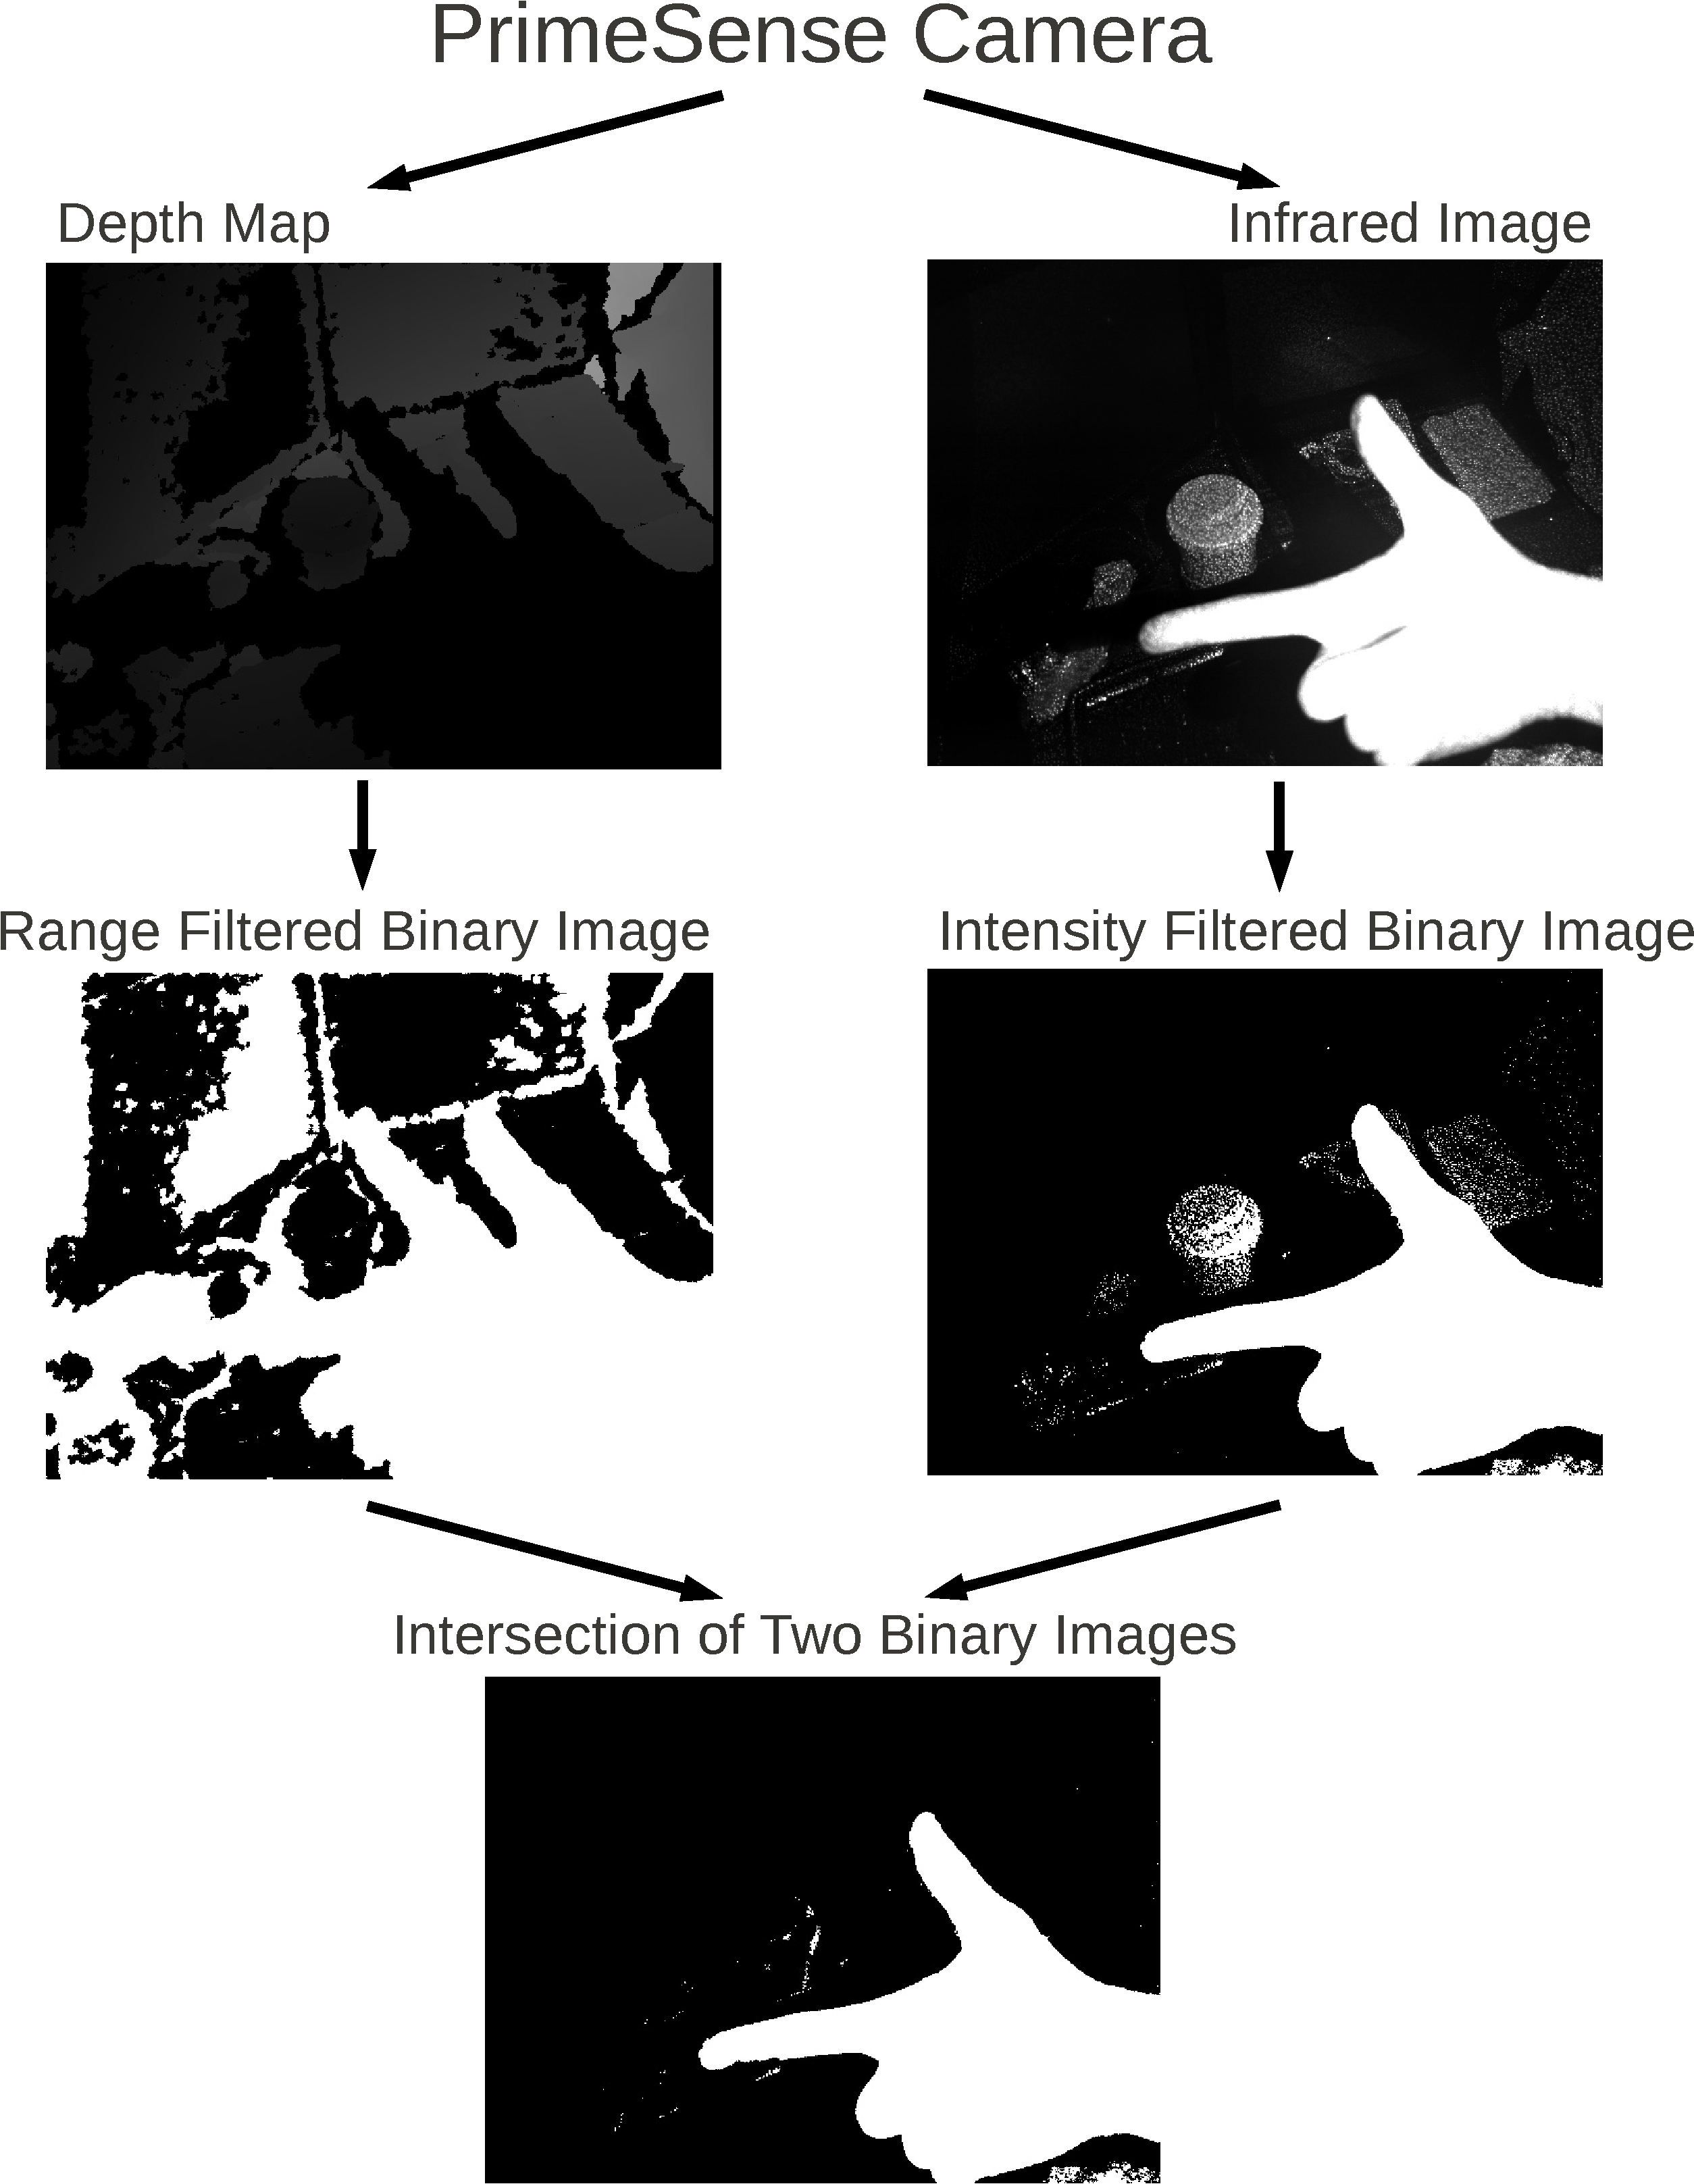
\includegraphics[width=0.8\columnwidth]{ch5/figs/crop_segmentation.pdf} 
\caption{Image segmentation steps. The binary image on the left has pixels
set to one if the depth map is unable to identify the object's relative
distance. The binary image on the right has pixels filtered out if lower than
threshold pixels, by setting them to zero. The intersection of the two
binary images becomes the image mask for gesture recognition. Notice that
there is still noise (e.g. outliers) present in the image mask. This happens
when both binary images fail to filter out the out-of-range pixels. For
example, a close distance (nearby) bright light source such as a bare tungsten
light bulb, strongly illuminated,
is both unidentified in the
depth map and is high in pixel values in the infrared image.
In other work we show how this problem can be solved using 3D HDR (High Dynamic
Range) imaging.}
\label{image_segmentation} 
\end{figure}

\begin{figure}
\centering
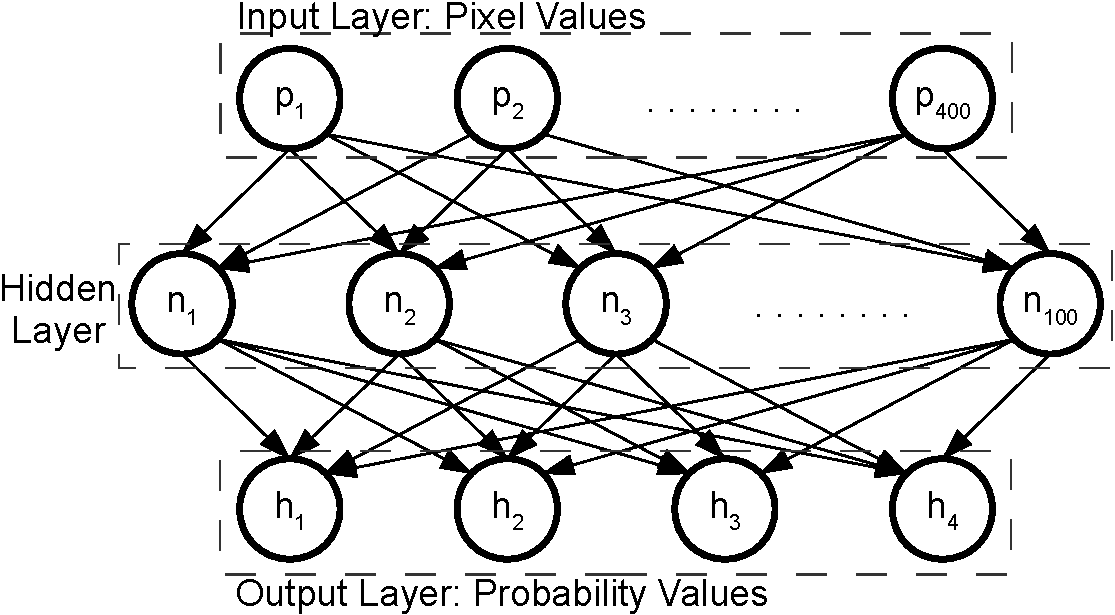
\includegraphics[width=\columnwidth]{ch5/figs/neural_net-crop.pdf}
\caption{The neural network implemented, takes 400 pixels at the input layer,
has 100 nodes in the hidden layer, and 4 output nodes. Each node represents
the confidence of the input being a specific gesture.}
\label{neural_net}
\end{figure}

\subsection{Classification}
We use a single layer neural network to achieve real time gesture recognition.
The extracted image mask of the hands is downsampled to a $20\times20$
pixels image. This image is fed into the neural network, and the neural
network outputs the probability of each gesture. Each pixel in this image
patch is treated as an input unit as shown in Figure~\ref{neural_net}.
Therefore, our input vectors to the neural network are always 400 to 1.
For the hidden layer, we choose to only implement 100 hidden units.
By choosing a small number for the hidden units, we are able to limit our
total parameter size to 40400. We decided this number is an efficient use of
computational resource for a real time recognition system on a wearable
battery-powered system. Finally, we have 4 output units since there are 4
different possible gestures we are interested in, as shown in
Fig~\protect\ref{gestures}. Each of these output units is the probability of
a unique gesture.
\begin{figure}
\centering
\begin{subfigure}[b]{0.25\columnwidth}
\centering
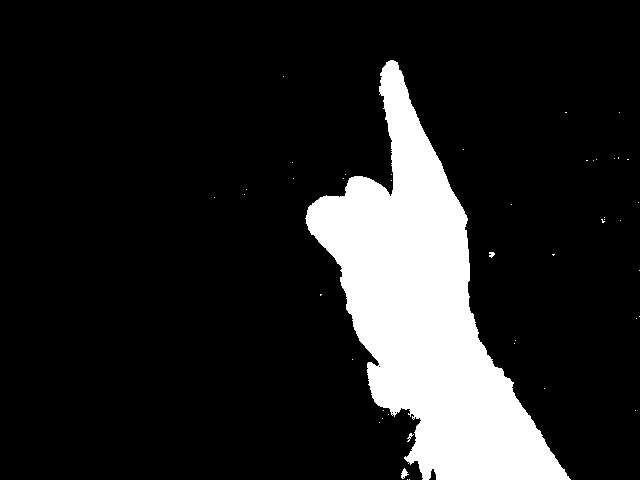
\includegraphics[width=0.95\columnwidth]{ch5/figs/pointing_up.png}
\caption{Point Up}
\end{subfigure}%
\begin{subfigure}[b]{0.25\columnwidth}
\centering
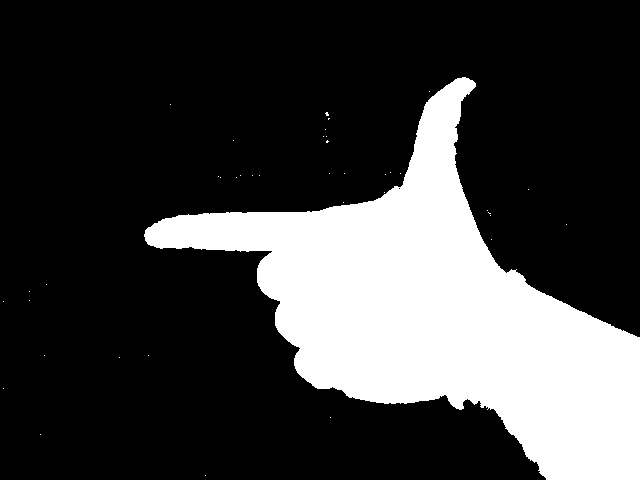
\includegraphics[width=0.95\columnwidth]{ch5/figs/lower_right_corner.png}
\caption{Lower Right}
\end{subfigure}%
\begin{subfigure}[b]{0.25\columnwidth}
\centering
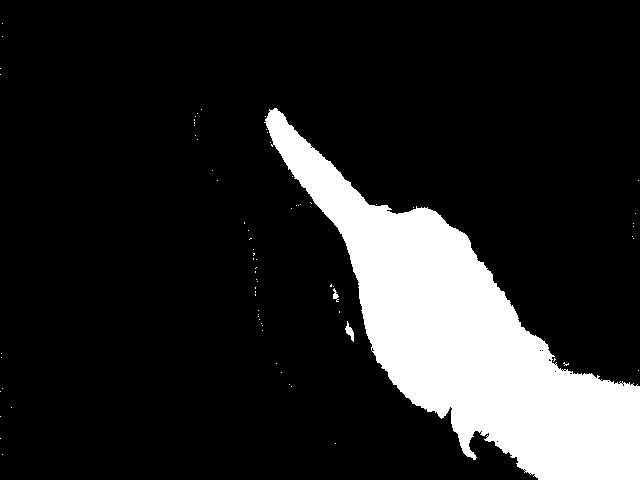
\includegraphics[width=0.95\columnwidth]{ch5/figs/point_angled.png}
\caption{Point Angled}
\end{subfigure}%
\begin{subfigure}[b]{0.25\columnwidth}
\centering
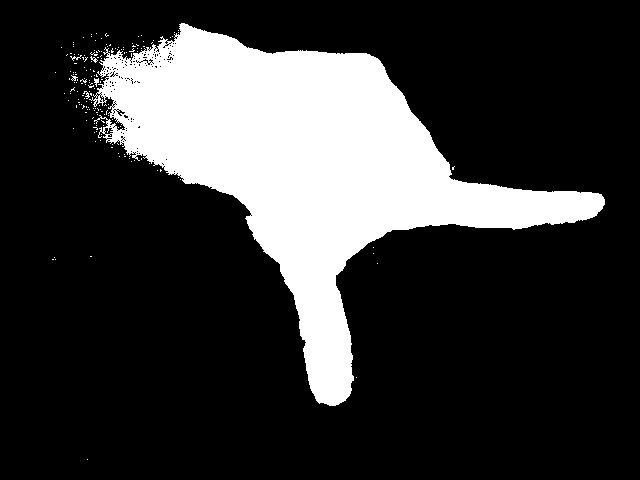
\includegraphics[width=0.95\columnwidth]{ch5/figs/upper_left_corner.png}
\caption{Upper Left}
\end{subfigure}
%\includegraphics[width=0.95\columnwidth]{ch5/figs/gesturesv2-crop.pdf}
\caption{Sample masked images of 4 gestures trained into the neural net.
During the classfication of each gesture, the system will recognize the
two gestures: point-angled and point-up as finger pointing. This helps
increasing the flexibility of gesture recognition for the users to post
gestures that are natural to them.}
\label{gestures}
\end{figure}

To train our neural network, we first needed to define the cost function. This
function is the log likelihood of a logistic regression. To find the best
possible parameters for the model, we needed to find the parameter which would
maximize this function. However, due to our gradient descent setting, we
negated the cost function to make it a minimization problem. Therefore, we are
trying to maximize the log likelihood function using minimization techniques.
To prevent over fitting to the training data, we introduced a regularization
term by adding the square of each parameter at the end of the cost function.
These regularization terms will ``punish'' the cost function as the parameters
become large, which can result in a floating point overflow. The training
cost function $J(\theta)$:
\begin{equation}
J(\theta) = l(\theta) + R(\theta, \lambda)
\end{equation}
\\
The term $l(\theta)$ is the logistic regression for minimization: 
\begin{equation}
\begin{split}
l(\theta) = -\frac{1}{s}\sum_{i=1}^{s} \sum_{j=1}^c 
& [y_j^{(i)}log(h_{\theta}(x^{(i)}))_j + \\
& (1-y_j^{(i)})log(1-(h_\theta(x^{(i)}))_j)]
\end{split}
\end{equation}
for which $s$ denotes the total number of training cases and $c$ denotes
the total number of output gestures. Since our objective of this function is
to add up the cost from each of our training cases. Thus, we use $i$ to
denote the current training cases that are being used to calculate the
cost. $h_{\theta}(x^{(i)})$ denotes the estimation resulted from the forward
propagation. After calculating the the estimate from forward propagation, we
use a logistic function to rescale that number between 0 and 1.
\\
The term $R(\theta, \lambda)$ is the regularization term: 
\begin{equation}
\begin{split}
R(\theta, \lambda) = \frac{\lambda}{2s}[ \sum_{i=1}^{n} \sum_{j=1}^{p} (\theta_{i,j}^{(1)})^2 + \sum_{i=1}^{c} \sum_{j=1}^{n} (\theta_{i,j}^{(2)})^2]
\end{split}
\end{equation}
for which $n$ denotes the total number of nodes in the hidden layer
and $p$ denotes the total number of nodes in the input layer, which is the
number of pixels we have in each of our training images.

\subsection{Training}
The training data were collected using the PrimeSense camera to record a
sequence of the image masks of various hand gestures. In particular, we focus
on the following gestures:
\begin{itemize}
    \item the framing gestures (consists of both hands that form the corners
          in diagonal of each other)
    \item the finger pointing gesture.
\end{itemize}

\subsubsection{Gesture Variation}
One problem associated with gesture recognition is that the the orientation
or form of a single gesture varies, with respect to the user and instance. 
Specifically, we consider two types of variations: the variations due to
change in orientation \cite{ren2011robust, uebersax2011real, li2009real} and
variations due to different forms of gesture that represent the same action. 

Figure \ref{gesture_data} shows some gestures that have the same meanings. The differences of these forms of gestures are not mere geometric transformation from one to another. To adapt to the form variations, we first define a group of different gestures that mean the same action. Each gesture of the same group is trained separately.

In addition to the form variations, we also attempt to train for the variations in orientation. This allows recognition system to adapt to slight angle changes of the hand. The inclusion of the variations helps the training to account for the gesture differences, which avoids limited recognition of only a single instance of the gesture.%
%
\begin{figure}
\centering
\begin{subfigure}[b]{0.33\columnwidth}
    \centering
    \begin{subfigure}[b]{\columnwidth}
    \centering
    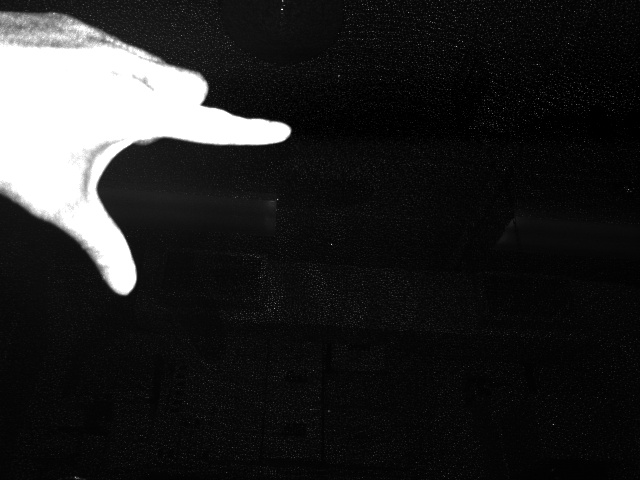
\includegraphics[width=0.98\columnwidth]{ch5/figs/upper_left_1.png}
    \end{subfigure}
    \\
    \vspace{1pt}
    \begin{subfigure}[b]{\columnwidth}
    \centering
    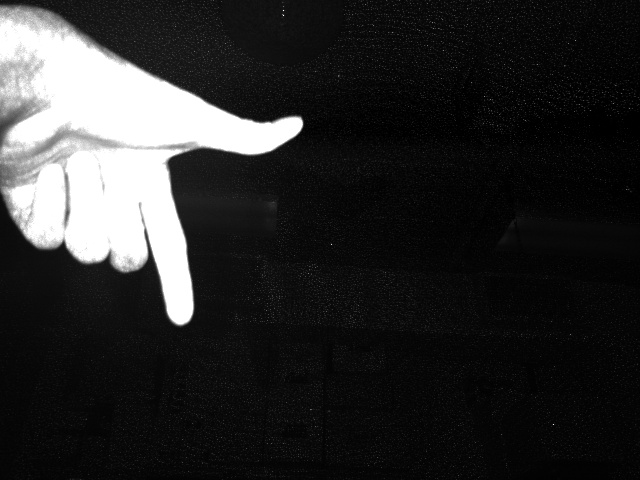
\includegraphics[width=0.98\columnwidth]{ch5/figs/upper_left_2.png}
    \end{subfigure}
    \caption{Upper Left}
\end{subfigure}%
\begin{subfigure}[b]{0.33\columnwidth}
    \centering
    \begin{subfigure}[b]{\columnwidth}
    \centering
    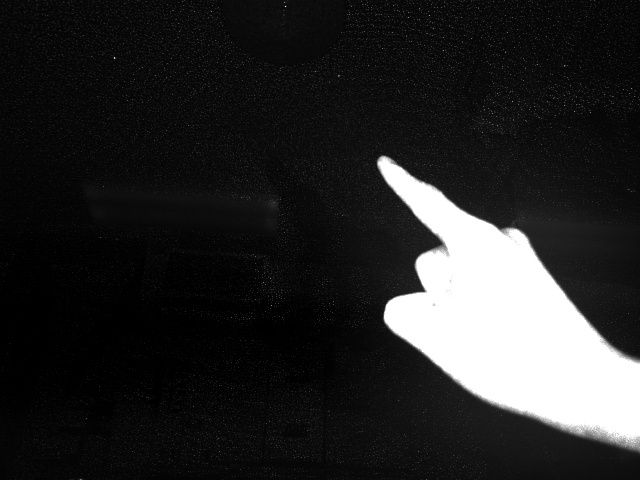
\includegraphics[width=0.98\columnwidth]{ch5/figs/point_angle_1.png}
    \end{subfigure}
    \\
    \vspace{1pt}
    \begin{subfigure}[b]{\columnwidth}
    \centering
    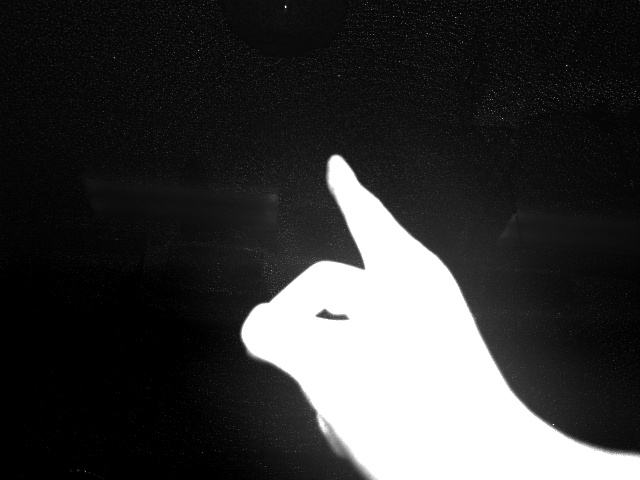
\includegraphics[width=0.98\columnwidth]{ch5/figs/point_angle_2.png}
    \end{subfigure}
    \caption{Point}
\end{subfigure}%
\begin{subfigure}[b]{0.33\columnwidth}
    \centering
    \begin{subfigure}[b]{\columnwidth}
    \centering
    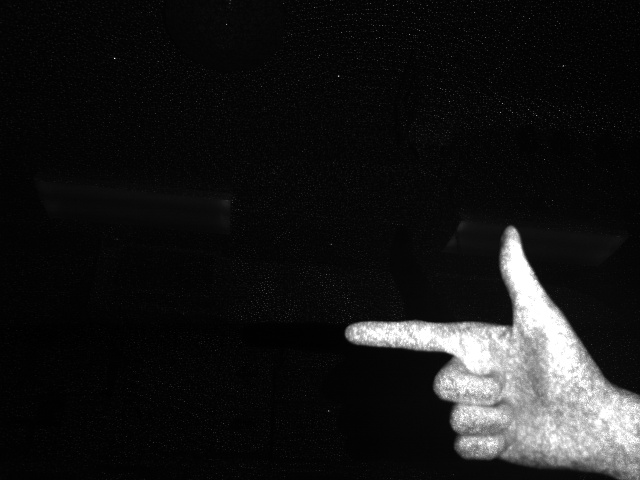
\includegraphics[width=0.98\columnwidth]{ch5/figs/lower_right_1.png}
    \end{subfigure}
    \\
    \vspace{1pt}
    \begin{subfigure}[b]{\columnwidth}
    \centering
    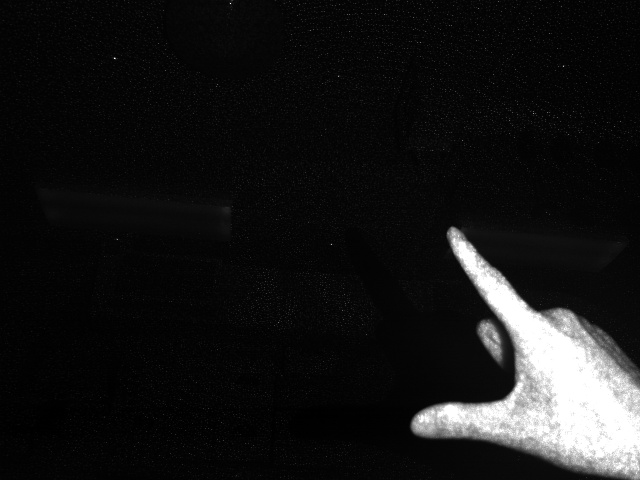
\includegraphics[width=0.98\columnwidth]{ch5/figs/lower_right_2.png}
    \end{subfigure}
    \caption{Lower Right}
\end{subfigure}
%\includegraphics[width=1\columnwidth]{ch5/figs/crop_training.pdf}
\caption{Demonstration of some of the gestures. The top row is one
instance of three different gestures and the lower row is examples
of alternative gestures for each of those in the top row.}
\label{gesture_data}
\end{figure}
%
\begin{figure}
\centering
\begin{subfigure}[b]{0.5\columnwidth}
\centering
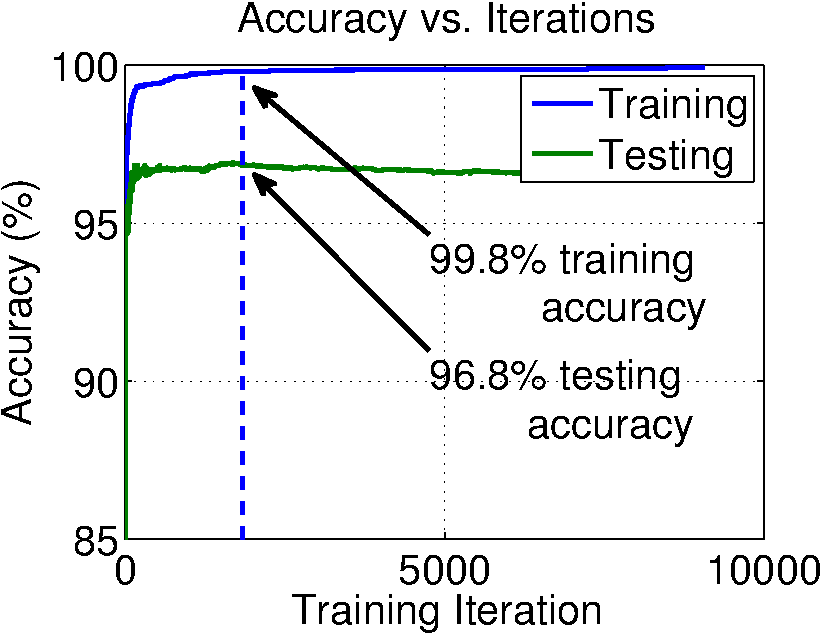
\includegraphics[width=\columnwidth]{ch5/figs/accu_vs_iter_f20.pdf}
\end{subfigure}%
%\\
%\vspace{10pt}
\begin{subfigure}[b]{0.5\columnwidth}
\centering
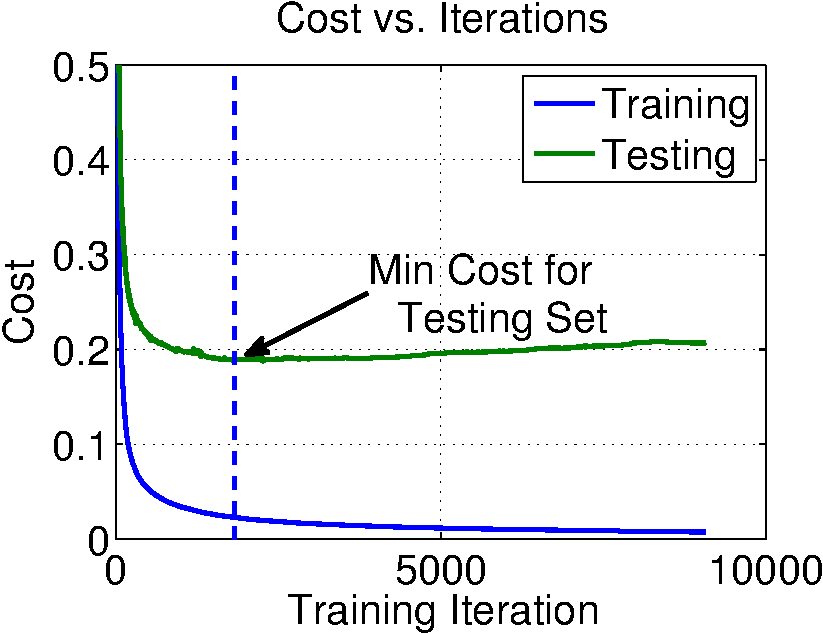
\includegraphics[width=\columnwidth]{ch5/figs/cost_vs_iter_f20.pdf}
\end{subfigure}
\caption{A graph of the Cost function versus Training iteration.
The graph shows the iteration at which to stop training the neural network
--- --- the minimum point of the testing cost.
Beyond this iteration, more training causes an increase in the testing cost.
At that iteration, the training set achieves a 99.8\% accuracy and the
testing set achieves 96.8\% accuracy.}
\label{stop_graph}
\end{figure}
\subsubsection{Data Collection}
Collecting a large amount of training data is one of the most effective way to improve the performance of a learning algorithm. In our setting, we could easily collect sample data by recording additional gesture samples in our daily use of the device. Although we are achieving high accuracy on our existing training data, we can constantly stream our gestures and label them with the correct label. This continuous data collection approach will keep improving our learning algorithm.

\subsubsection{Early Stopping}
In order to avoid over fitting to our training data. We separated 80\% of our data as our training data and 20\% of our data as test data. On every iteration of neural net training, we run  forward propagation to get our gesture prediction accuracy and cost on both training and test set. We plot the cost on both training and test sets versus the number of training iterations as shown in Figure~\ref{stop_graph}. As you can see in the Figure~\ref{stop_graph}, at around iteration 2000, the cost of the test data starts to increase while the cost of the training data is still decreasing. This implies that after approximately 2000 iterations, our neural net is being over trained to the training data, that is, if left to train forever, the neural network will only match items in the training data and reject everything else.

\section{Proposed Hardware and Implementation}
In this project, our goal is to create and implement an augmediated reality system using gesture recognition as a user interface. To achieve this, we utilize the 3D sensors (ASUS Xtion / SoftKinetic) to observe the world and gestures from a first person view (see Figure~\ref{fig:3Dcamera_head} and~\ref{fig:wearable_qr}). The ASUS Xtion is a PrimeSense based range camera which provides depth maps and infrared images of the scene it is observing. This camera uses an infrared projector and infrared camera to determine the depth map. The images are processed in real time with an ODROID-X2, which is an ARM-based mobile development platform with a 1.7GHz ARM Cortex-A9 Quad Core processor. Finally we display the result using the Epson Moverio BT-100. 
%\subsection{Epson Moverio BT-100}
The Epson Moverio BT-100 is a head-mounted display that uses a transparent screen. Based on the principles discussed in \cite{mann2001wearable}, Epson's Moverio is a good candidate for mediated reality applications due to its special display, which allows users to interact with the physical world with less eye straining issues. The Moverio is capable of streaming from an external video source and was therefore used as a display for the processed information from the range camera. In this project, we processed the range camera information with ODROID-X2 and added additional mediated reality information to the Moverio. The user will see a mediated reality, such as a mediated user gesture interface, that will interact with real world object.

\begin{figure}
\centering
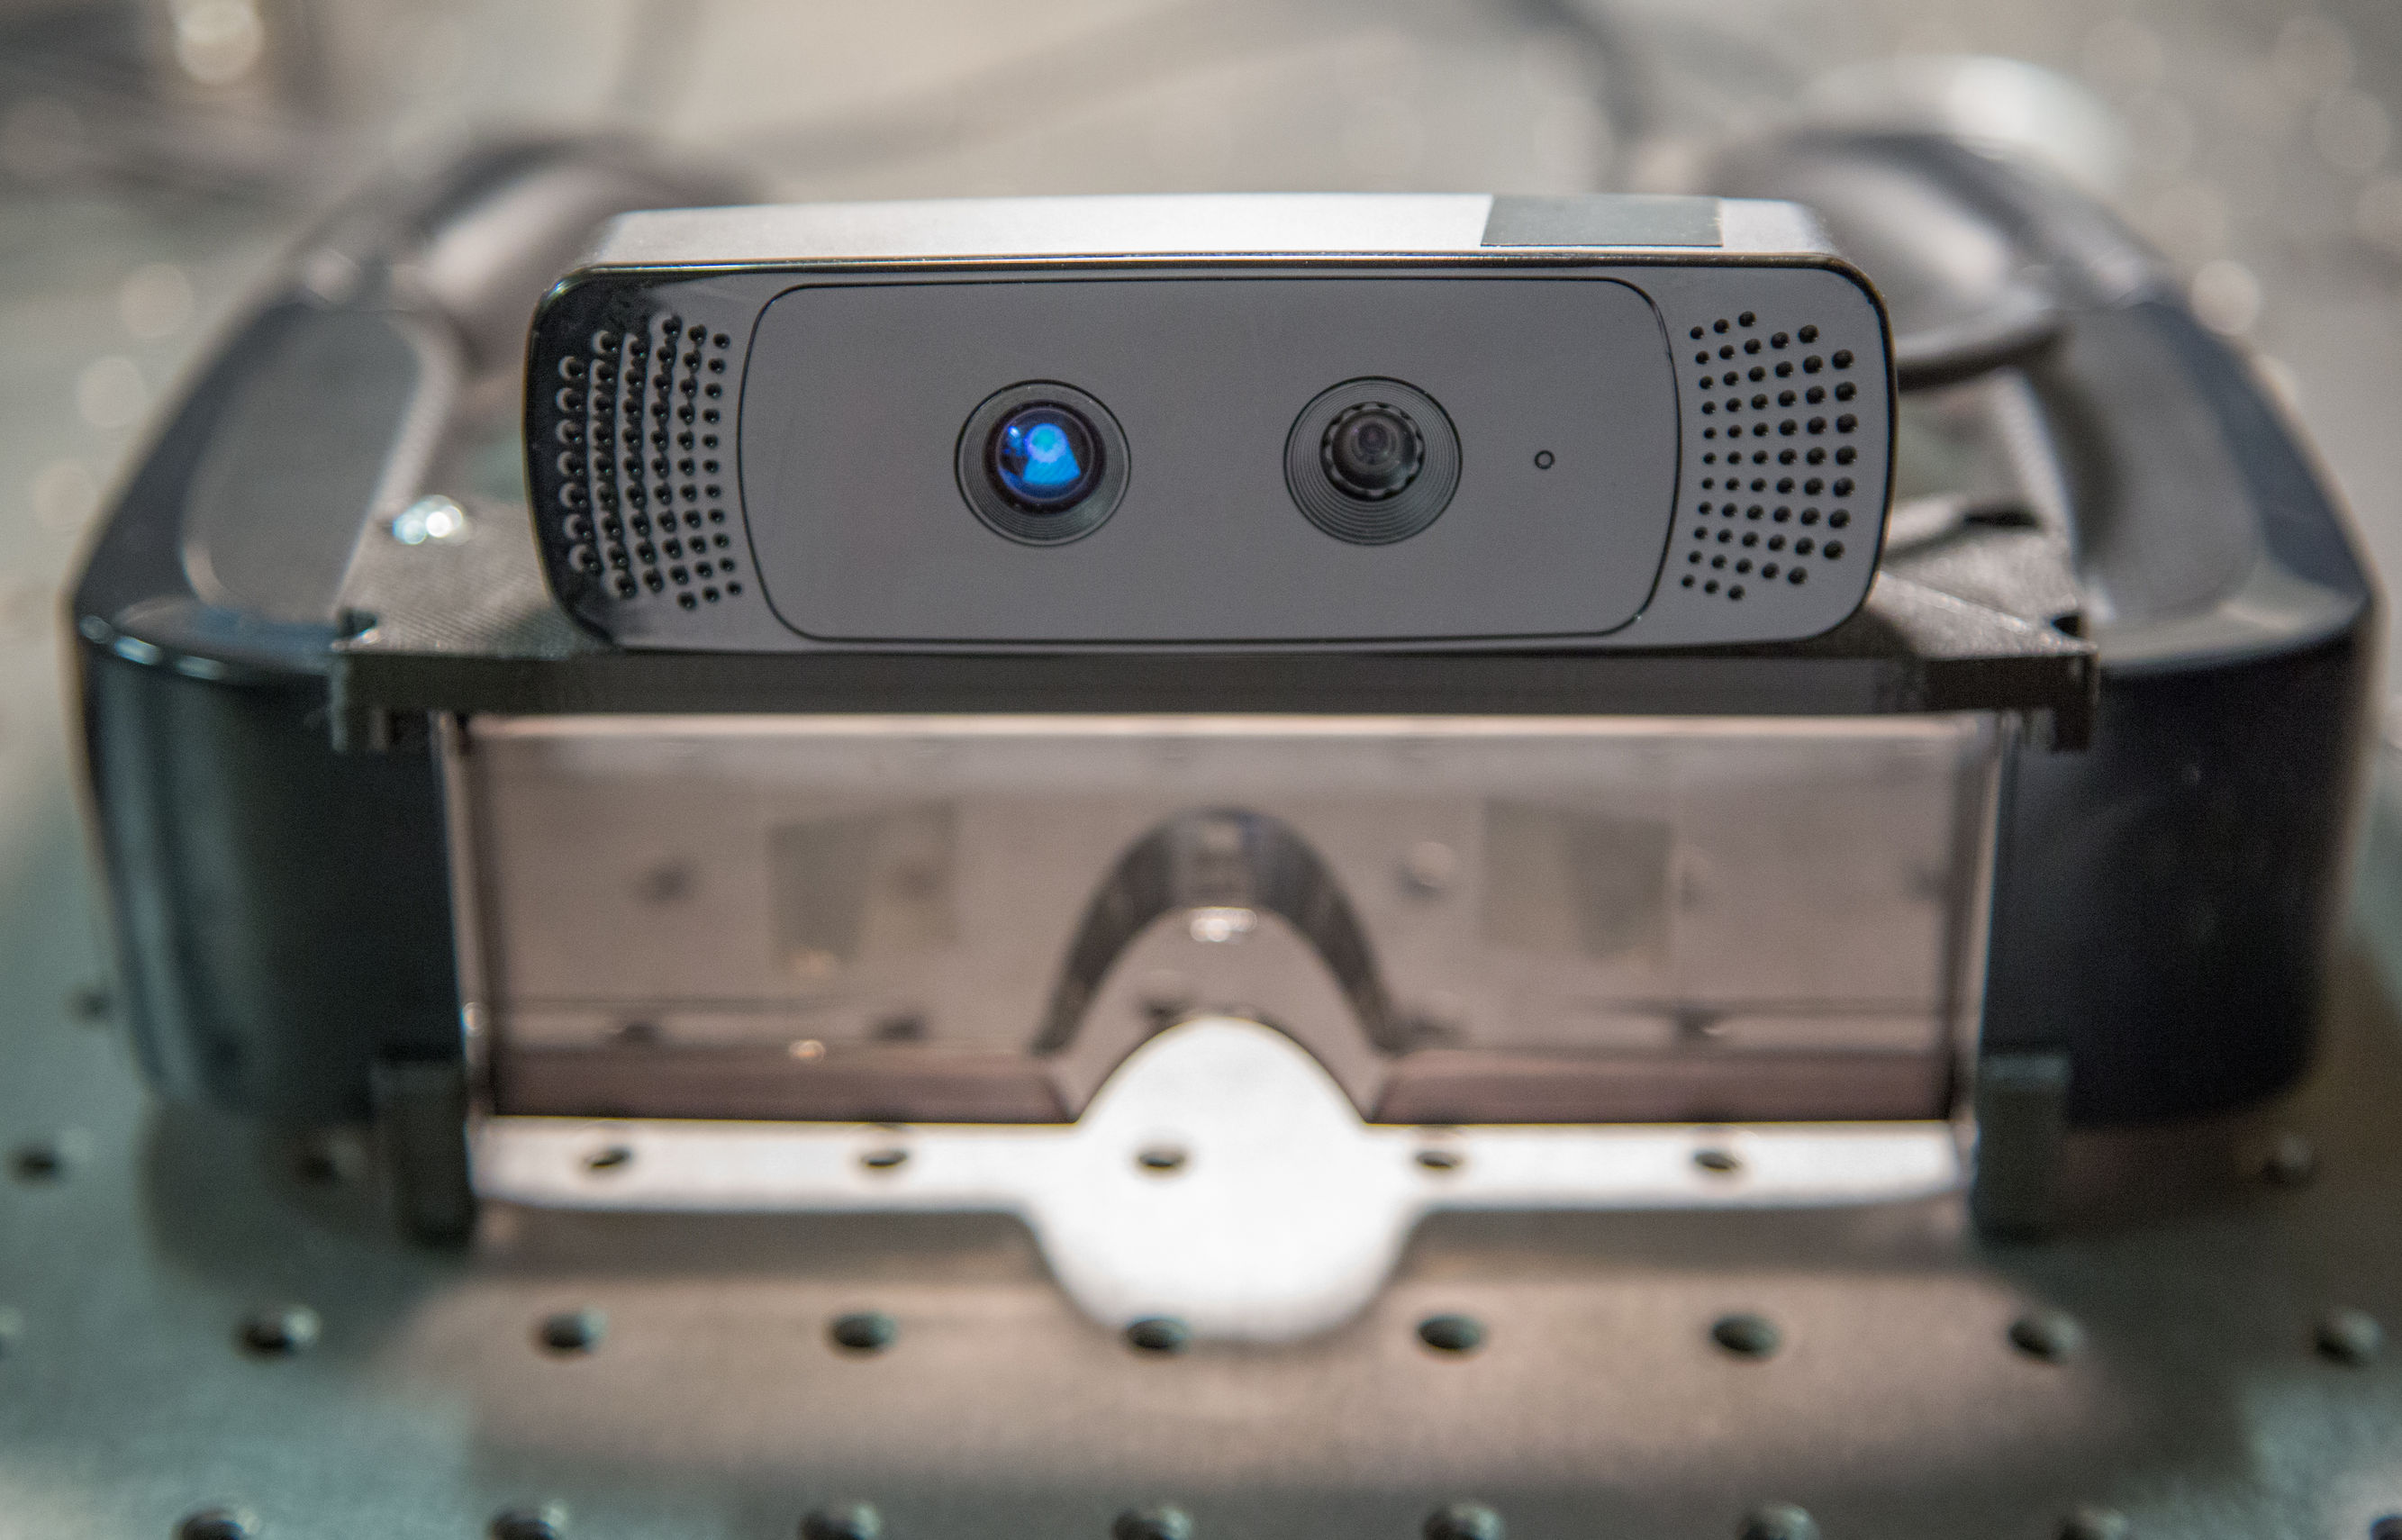
\includegraphics[height=1.8in]{ch5/figs/wearable/low_res/eyetap_mann_glass.jpg}
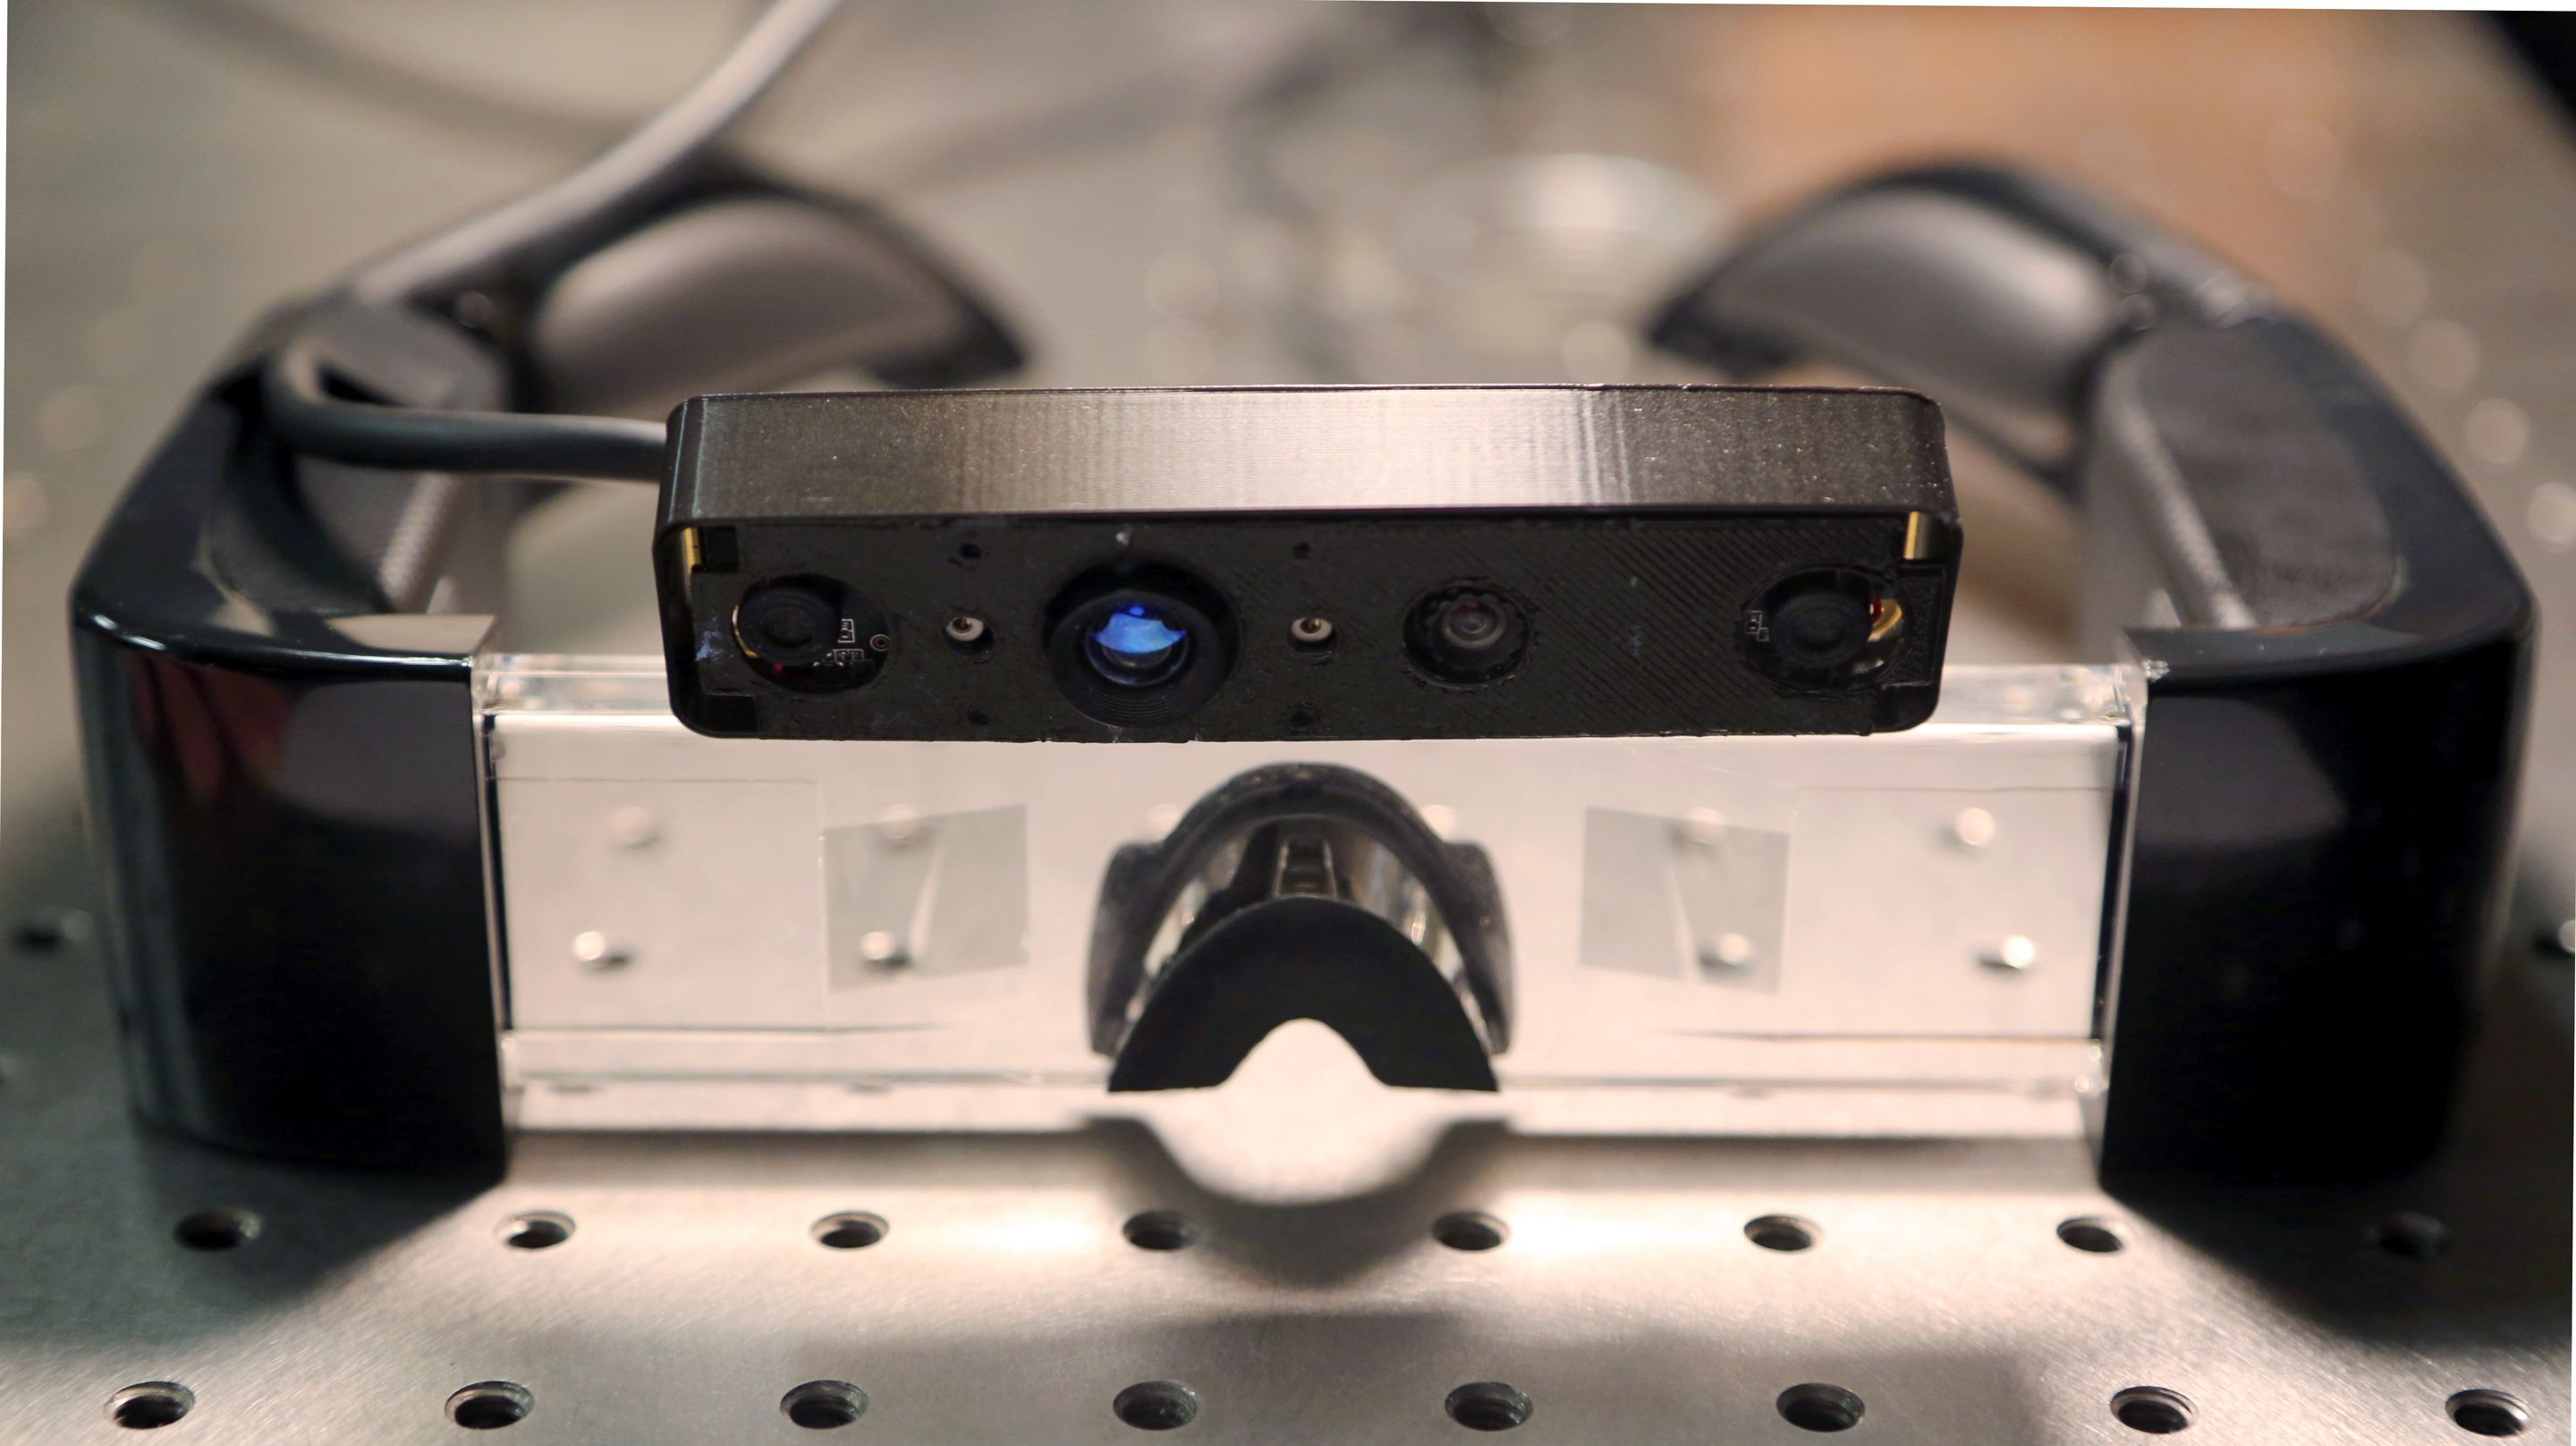
\includegraphics[height=1.8in]{ch5/figs/wearable/low_res/eyetap_slim_IMG_2408.jpg}
\caption{Example of FreeGlass which combines the 3D sensing camera from SoftKinetic
and the transparent digital eye glass display from EPSON. The camera is mounted onto the eye glass with our custom 3D printed parts. 3D camera mounted in our custom enclosure to reduce size and weight. }
\label{fig:3Dcamera_head}
\end{figure}

\subsection{Performance}
The training stage of our neural network achieved an accuracy of 99.8\%. The cross-validation of the trained neural network achieved an accuracy of 96.8\%. The performance in frames-per-second (FPS) of only the gesture recognition on the ODROID-X2 is approximately 100 FPS while the performance of the complete wearable system, including gesture recognition, is approximately 30 FPS.

\section{Applications}
Our proposed wearable eyeglasses system enables users to perform gesture-based control in everyday life. Unlike other mobile devices, our system is always-ready and it continuously processes information about the environment. Such a feature enables novel applications, such as interactive QR-based infographic interface, which automatically acquires/mediates information about our environment and require minimum user intervention. Furthermore, the camera system also brings forth social implications that arises with other camera-enabled systems.

%\subsection{First Person View Gesture Recognition Based User Interface}
\subsection{Augmediated Reality Interface with Real Physical Objects}
The wearable 3D eyeglasses and 3D range sensors provide an novel interface for an immersive interaction with the physical world. Instead of solely based on augmented reality, which only add augmented elements in to the real world scene, our gesture recognition system along with the wearable 3D glasses can efficiently detect the surrounding environment and perform augmediated application, which involves adding and subtracting information in the real world scene and enable more interactivity between the user and computer. Users are able to see the real world environment along with the user interface. In Figures \ref{select_off} and \ref{select_on}, the user is able to toggle a $Select$ function by overlaying his/her `finger pointing gesture' over the $Select$ button.  Unlike traditional devices, where the users have to control the device with their hands, our approach gives the user a more intuitive and hands free control over the device.

\begin{figure}
    \centering
    \begin{subfigure}[b]{0.5\columnwidth}
        \centering
        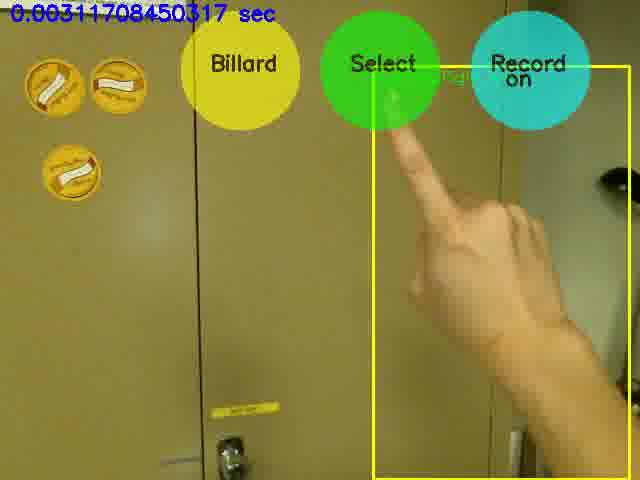
\includegraphics[width=\columnwidth]{ch5/figs/28}
        \caption{$Select$ OFF}\label{select_off}
    \end{subfigure}~\begin{subfigure}[b]{0.5\columnwidth}
        \centering
        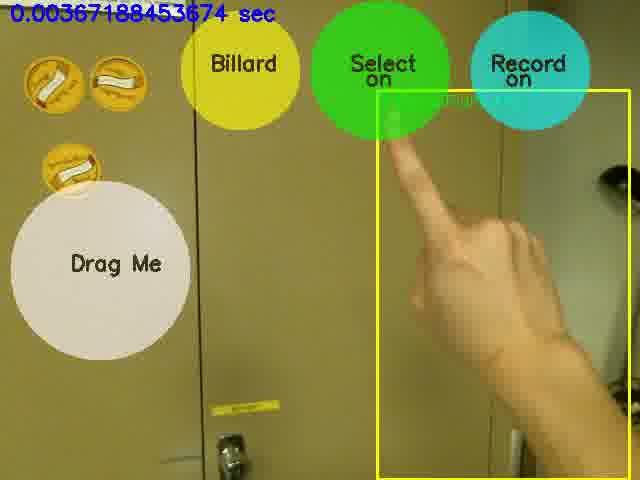
\includegraphics[width=\columnwidth]{ch5/figs/29}
        \caption{$Select$ ON}\label{select_on}
    \end{subfigure}
    \\
    \vspace{10pt}
    \begin{subfigure}[b]{0.5\columnwidth}
        \centering
        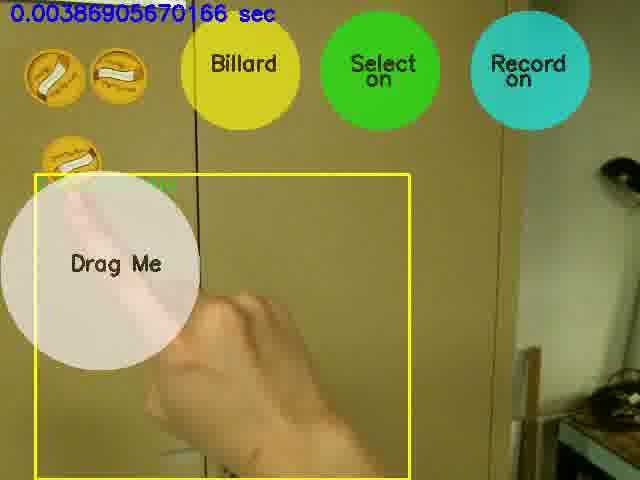
\includegraphics[width=\columnwidth]{ch5/figs/45}
        \caption{Initiating $Drag Me$}\label{drag_init}
    \end{subfigure}~\begin{subfigure}[b]{0.5\columnwidth}
        \centering
        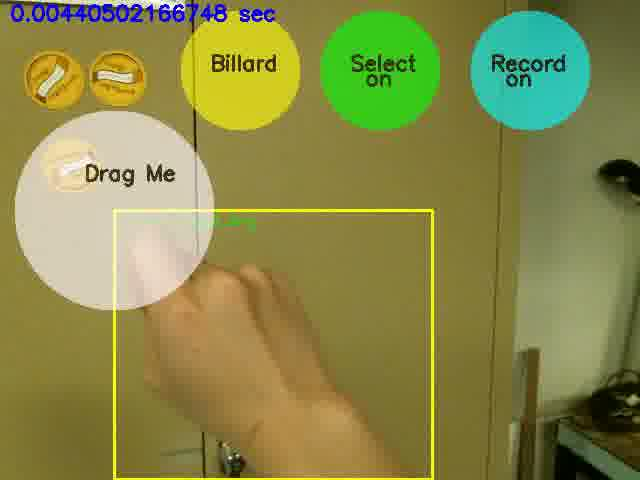
\includegraphics[width=\columnwidth]{ch5/figs/46}
        \caption{Moving $Drag Me$}\label{drag_me}
    \end{subfigure}
    \caption{Some sample interactions using the wearable gesture recognition system. Fig \ref{select_off} and Fig \ref{select_on} shows a gesture toggling a virtual-button. Fig \ref{drag_init} and Fig \ref{drag_me} shows a gesture moving a virtual object in the scene.}
\end{figure}

\subsection{(Mediated) Reality Window Manager}
(Mediated) Reality Window Manager (RWM) is another important application for our gesture recognition system. Users are able to drag around an augmented window as you can see in Figures \ref{drag_init} and \ref{drag_me}. This window can contain various information such as conference calling, web pages and GPS maps. This application allows user to do their daily desktop/laptop environment task directly in a first person mediated reality window.

\begin{figure*}
\centering
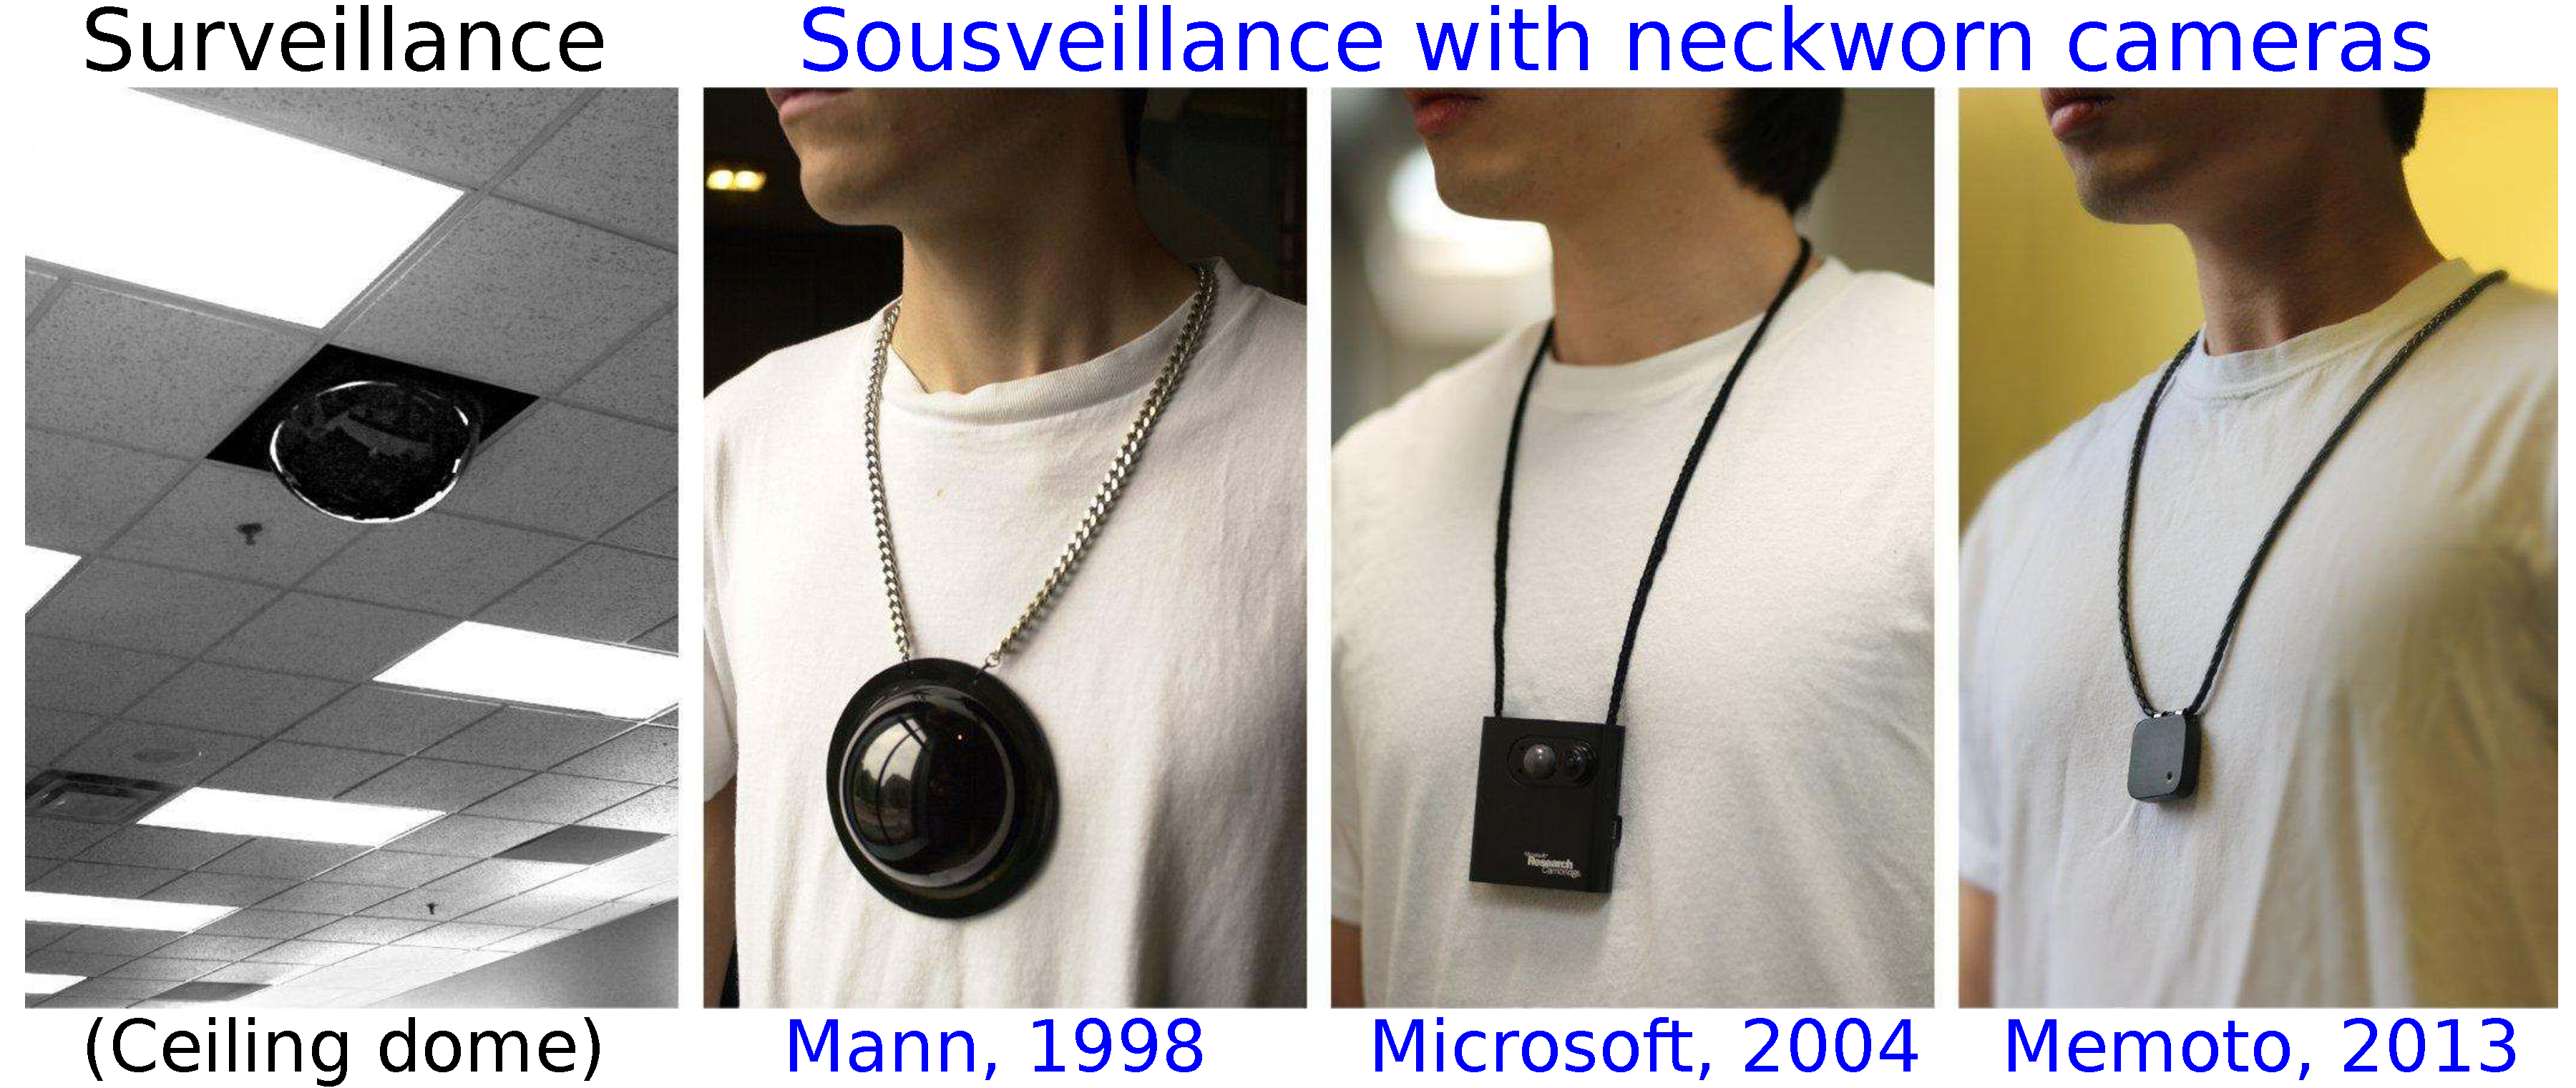
\includegraphics[width=6in]{ch5/figs/coop_surveillance_sousveillance_fixed_with_vi.pdf}
\caption{Neckworn camera systems for first-person sensing.
         Leftmost: Surveillance camera picture (taken in 1994) was the original
         source of inspiration.} 
\label{neckcams} 
\end{figure*}

\begin{figure*}
\centering
{\includegraphics[width=5.8in]{ch5/figs/6ense_low_res.pdf}}
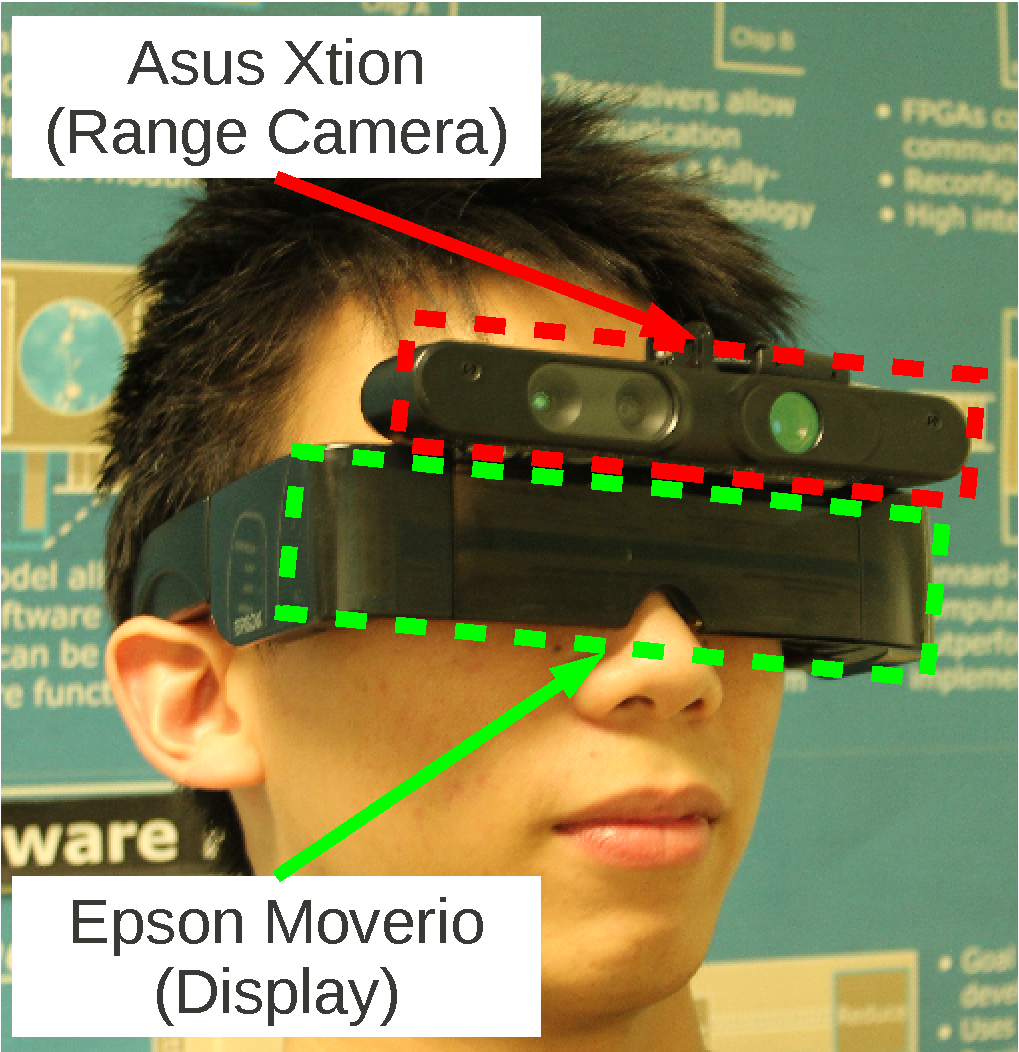
\includegraphics[height=2.5in]{ch5/figs/crop_wearable}
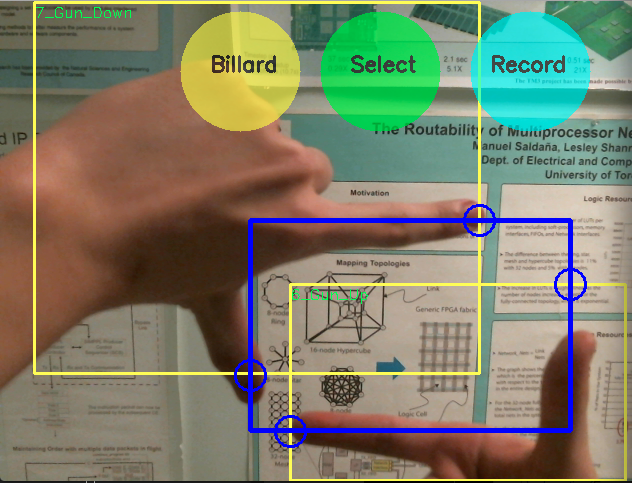
\includegraphics[height=2.5in]{ch5/figs/bounding_box.png} 
\caption{Gesture-based wearable computing.
Leftmost: Two examples of ``Synthetic Synesthesia of the Sixth Sense''\cite{mann2001cyborg},
commonly abbreviated as ``Sixth Sense'' or ``SixthSense'' which is a wearable
computing system with various sensors.  The system pictured here is
capable of augmented reality without the need for eyewear.
The system was originally built into a surveillance dome,
to mimick the form of the ceiling dome concept of
Fig~\protect\ref{neckcams}.
Other variations of SixthSense
utilize a finger marker and RGB camera to capture the gestures
in order to project augment reality frames
on a surface~\cite{mistry2009sixthsense}.
Rightmost: In addition to Augmented Reality,
FreeGlass also allows Augmediated Reality, i.e. a partially mediated reality
that can, within the limits of the dark shade, selectively augment or diminish
various aspects of the scene.
Here for example, the
system recognizes a two-corner gesture to overlay a bounding box (blue frame)
on top of the wearer's view. The blue circles indicate the location of the
finger tips. An application of such a gesture is to select a region
of interest from the wearer's view.} 
\label{bounding}
\label{6sense} 
\end{figure*}

\subsection{Region of Interest Selection With Gesture}
In most image based object recognition tasks, it is often difficult to determine which object of interest in a photo a person would like to classify on without any user inputs. To reduce the search area for object classification, methods such as eye tracking \cite{schiessl2003eye} and hand gestures are natural ways for the user to inform the system where the user's focus is. For example, if the scene contains a chair and a table and the person wants to see the price of that chair, without any additional indication from the user, the recognition system may only attempt to retrieve the price information of both items and display them. With the gesture recognition enabled in the system, the user is able to guide the system to a specific object of interest. This is done by first constraining the area of the view using the bounding box to bring forth the region of interest. The user may naturally select the region of interest by posting two-corner gesture, as seen in Figure \ref{bounding}.

In addition to utilizing our gesture recognition system as a preprocessing tool for object recognition, we integrate the use of QR (Quick Response) code to improve the accuracy of object recognition and to speed up recognition performance. QR code has been used extensively over the past few years in terms of advertising on mobile platforms due to its simplicity, robustness, and speed. People can look at a poster and scan the QR code and get redirect to the event website. In our wearable gesture recognition setting, it provides a natural experience when working with QR code technology. A user can be walking down the aisle in a grocery store and acquire product information by scanning QR codes. To activate the QR code and get additional information on the products such as ratings, the user can perform a gesture command to segment out the QR code of the interested product. Once the QR code is segmented and recognize, our wearable system will send a request to a URL and display the corresponding information. 

%\subsection{3D Gestures with Multiple Eyeglasses}
%With a multiple users and eyeglasses, we propose an novel application which allows users to share a mediated reality space in real-time based on gesture controls using 3D cameras. The 3D cameras in our system 
\begin{figure*}
        \centering
        \begin{subfigure}[b]{0.5\textwidth}
                \centering
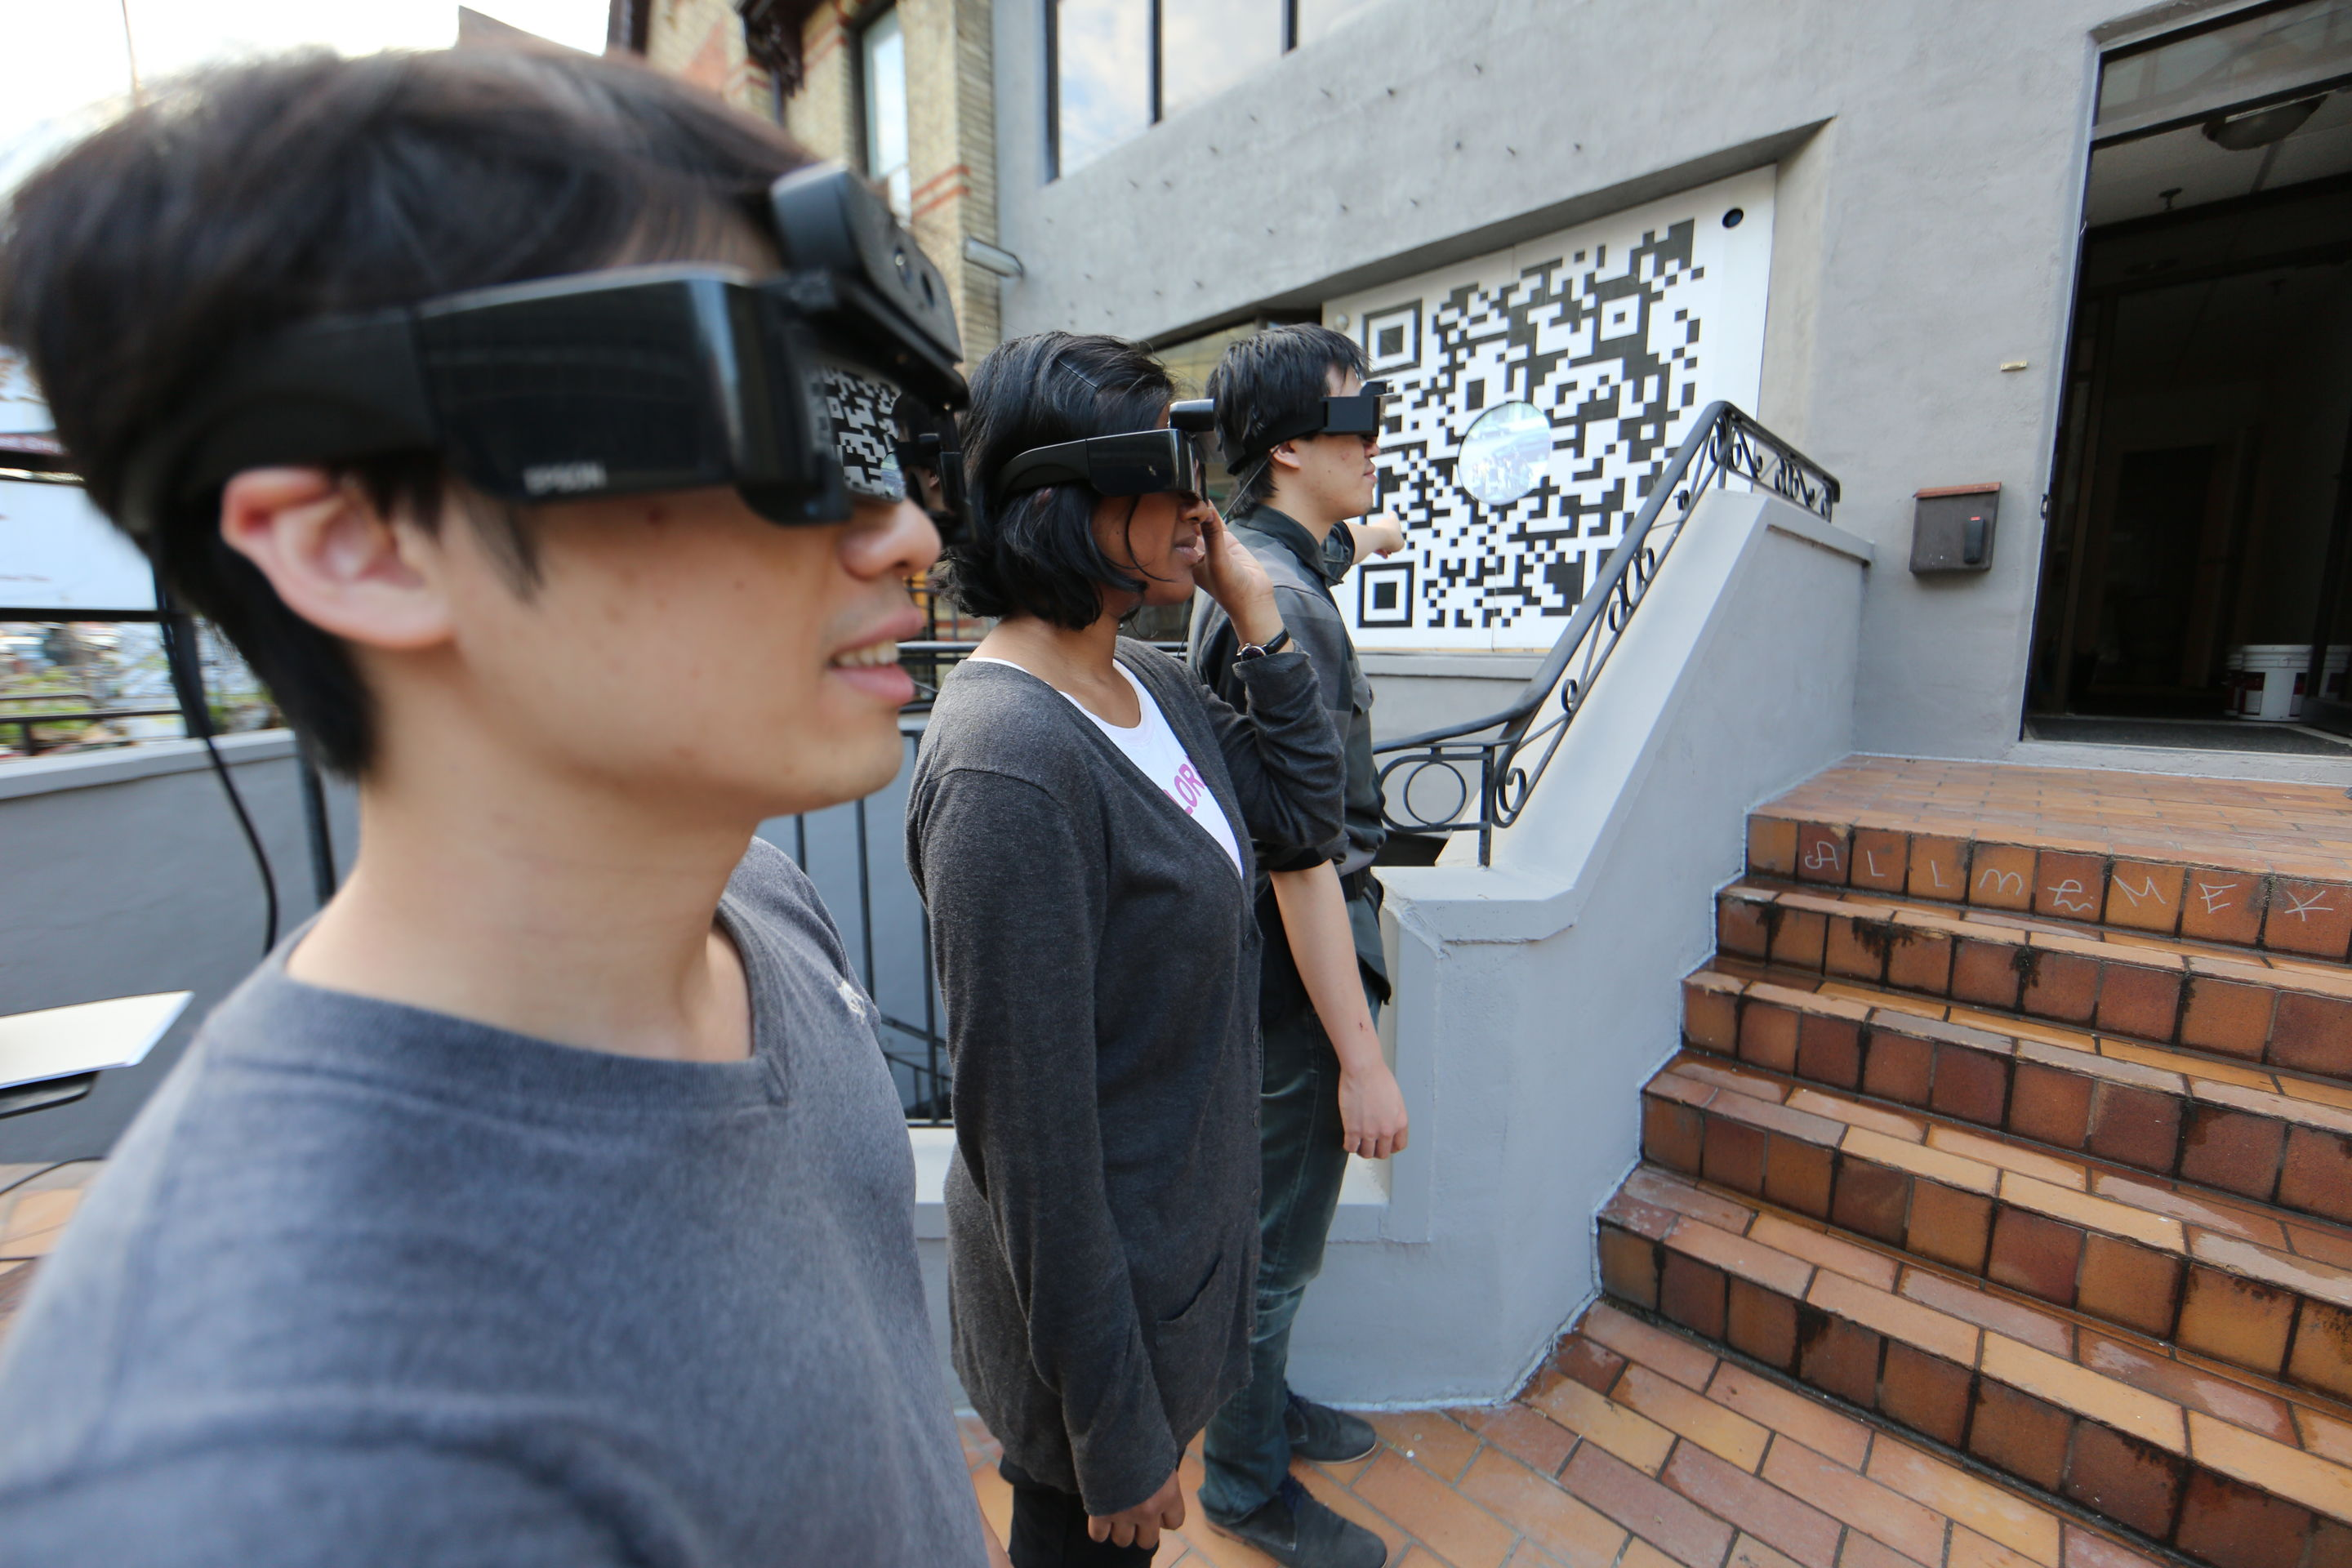
\includegraphics[height=2in]{ch5/figs/wearable/low_res/3_eyetap_qr_line_IMG_2232.jpg} 
                \caption{}
                \label{fig:qr_wall}
        \end{subfigure}%
        %add desired spacing between images, e. g. ~, \quad, \qquad etc.
          %(or a blank line to force the subfigure onto a new line)
        \begin{subfigure}[b]{0.5\textwidth}
                \centering
		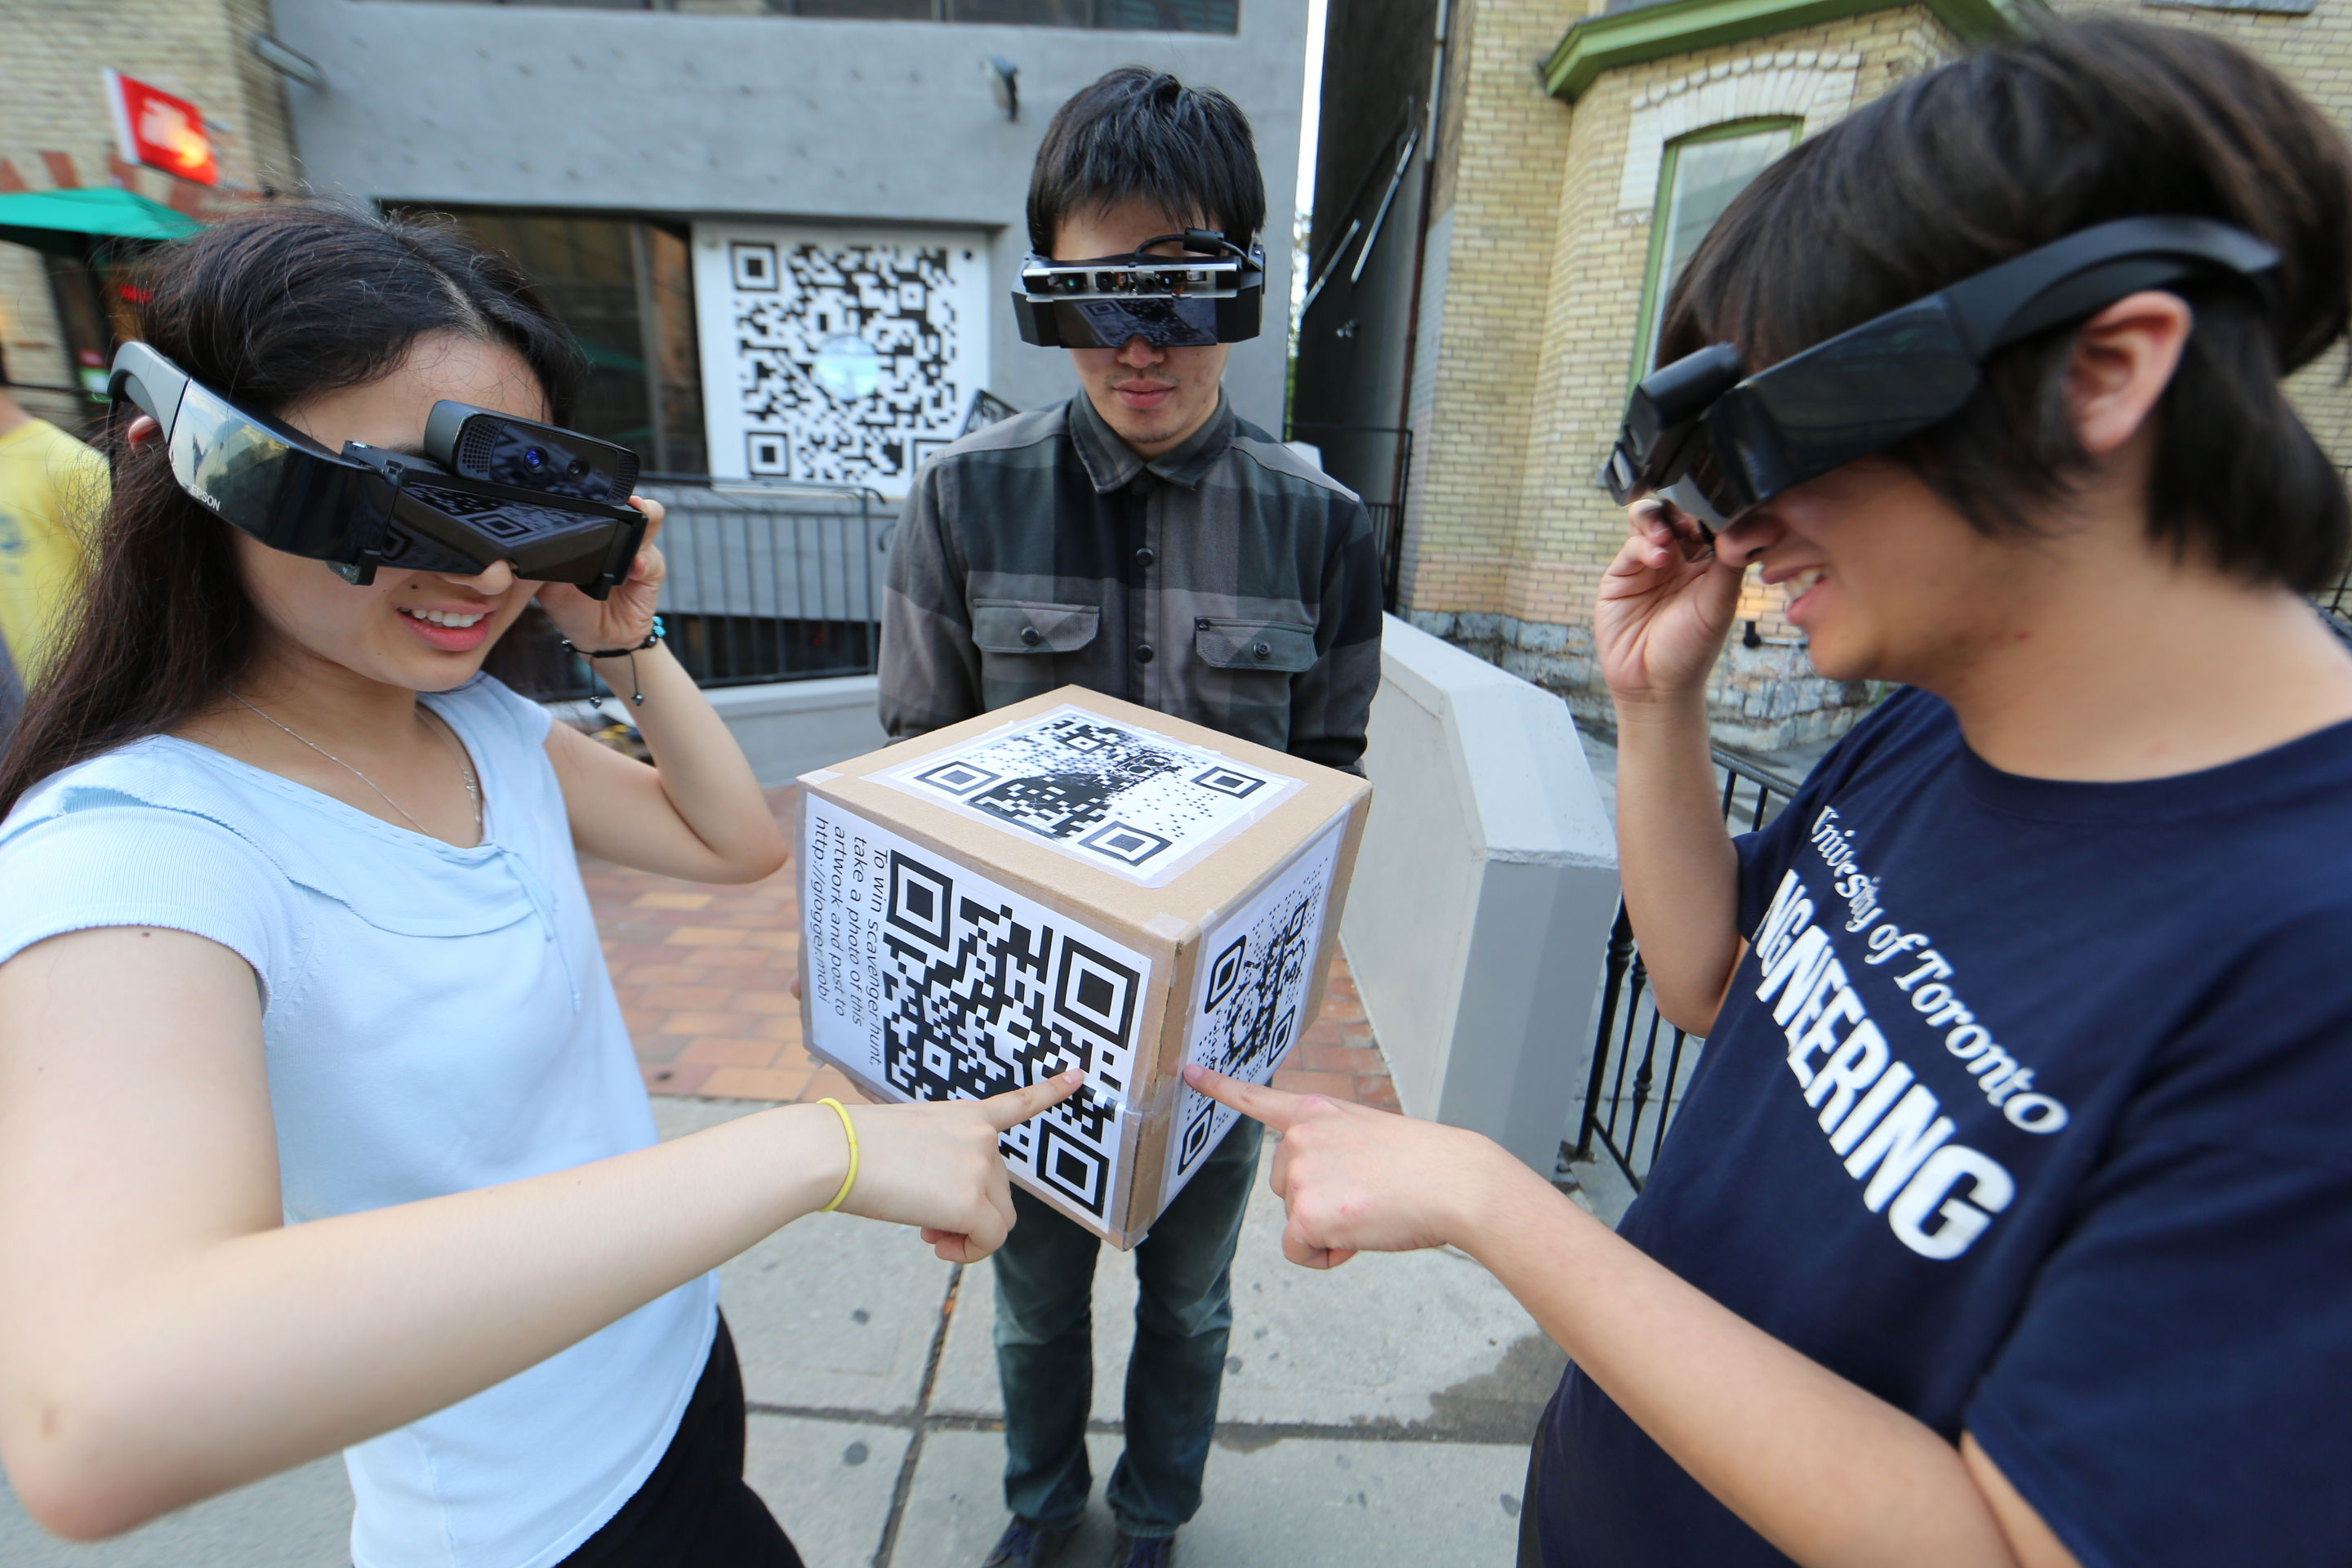
\includegraphics[height=2in]{ch5/figs/wearable/low_res/3_eyeglass_3_IMG_2303.jpg} 
               \caption{}
                \label{fig:qr_cube}
        \end{subfigure}
        
        %add desired spacing between images, e. g. ~, \quad, \qquad etc.
        %(or a blank line to force the subfigure onto a new line)
        \begin{subfigure}[b]{\textwidth}
                \centering
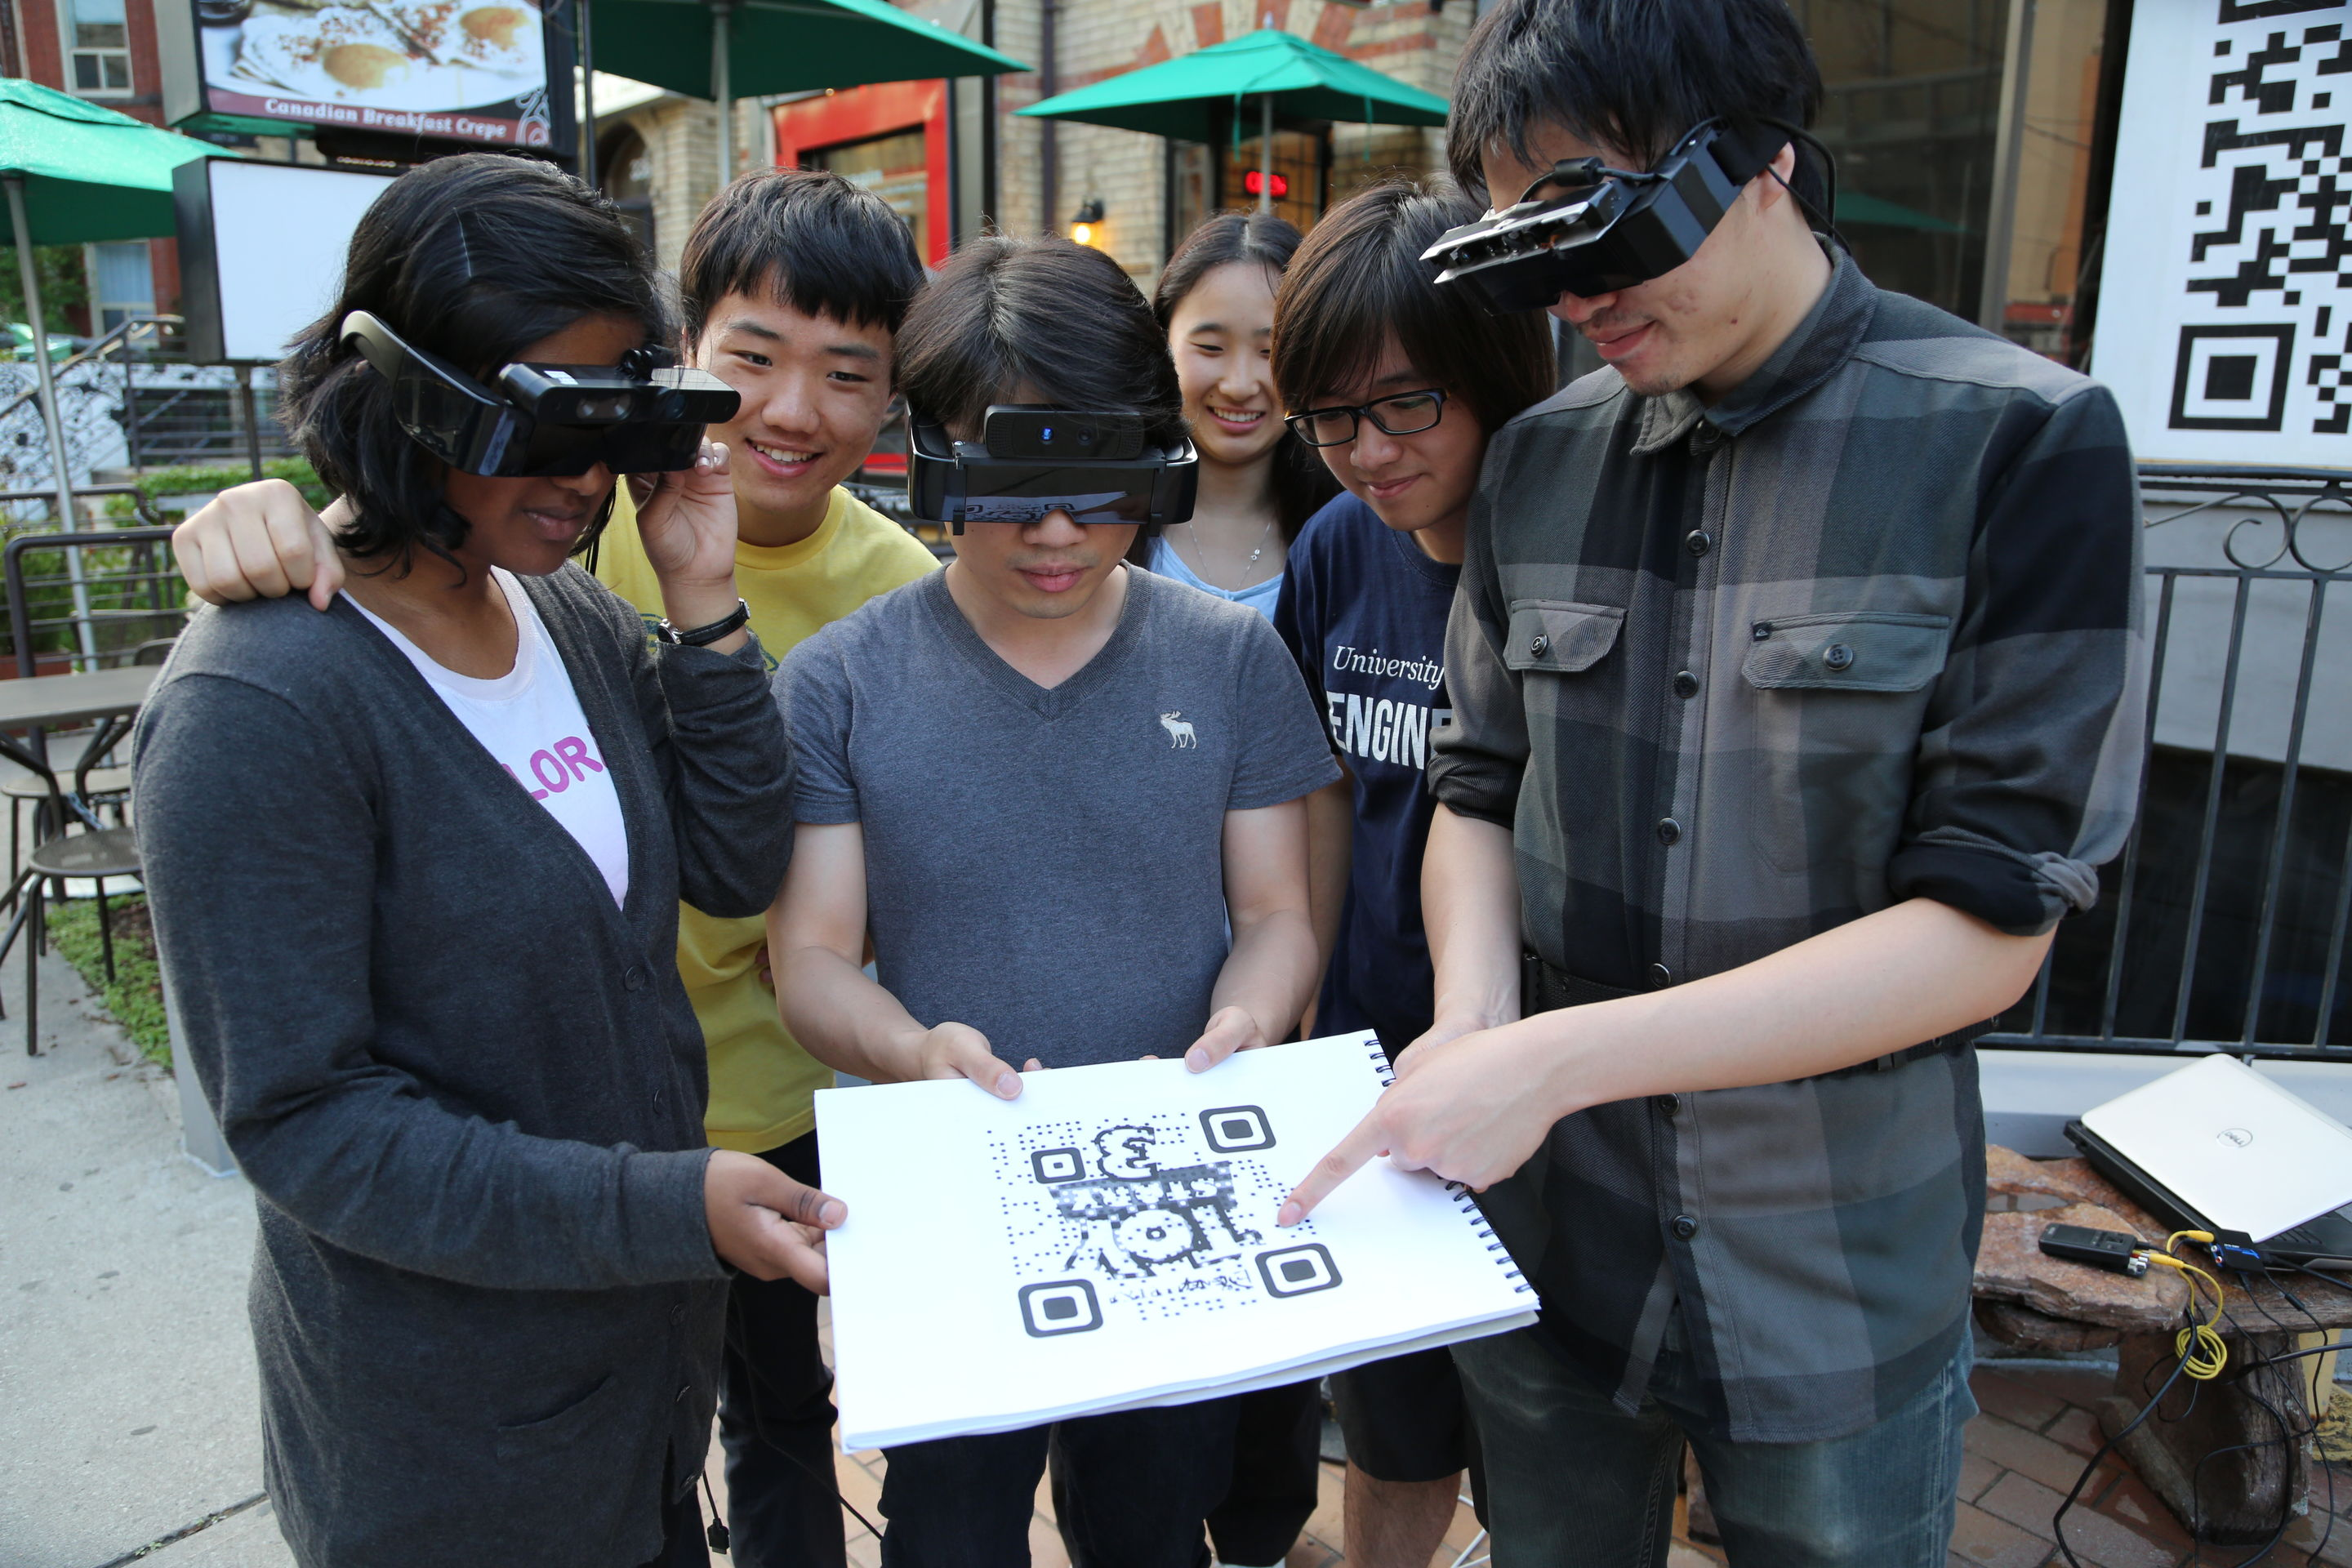
\includegraphics[height=4in]{ch5/figs/wearable/low_res/3_eyeglass_paper_2_IMG_2175.jpg} 
                \caption{}
                \label{fig:qr_paper}
        \end{subfigure}
        
        \caption{Applications of the collaborative gesture-based interface among multiple eyeglasses. Our proposed hardware system allows multiple users to interact with real physical objects, such as QR code on the building, sketchbook, or boxes. Users experience a shared of virtual and physical space through the eyeglasses, and our gestures interface provides an intuitive methods for real-time interaction.}\label{fig:wearable_qr}
\end{figure*}

\section{Social Implications}
Wearable Computing devices provide a revolutionary form of personal assistance, augmented reality/mediated reality and the like \cite{hill2004reality,aimone2003eyetap}.

Serendipitous gesture recognition on a mobile wearable device requires
constant sensing of the environment. For example, the vision based
wearable gesture recognition system (Figure~\ref{fig:wearable_qr})
continuously processes
every frame of incoming video so that the system is ready to recognize any
hand gesture when it occurs.  FreeGlass might remain dormant for an
extended time, and then be ``awakened'' by a simple hand gesture that
gives commands corresponding to the
gesture the system recognizes.
By definition, this particular setup will be
classified as a sousveillance system \cite{mann2004sousveillance,mann2006cyborglogging,mann2002sousveillance}, which is the opposite of
surveillance, i.e. instead of a camera system mounted to a building,
the camera is human-centric, and the world through this device is
captured as a first person view.  There has been recent
debates over the appropriate use of sousveillance devices
such as EyeTap, MannGlass, and Google Glass. On one hand, some people see
sousveillance devices as a threat to personal privacy that should
be forbidden.  But many spaces already use surveillance, and as such,
sousveillance is seen by many as creating a necessary balance in an otherwise
one-sided ``surveillance society''.

Moreover, many business and retail establishments use
surveillance cameras themselves but prohibit others from
bringing their own cameras or cell phones.  See Fig~\ref{surveillancehypocrisy}.
\begin{figure}
  \centering
  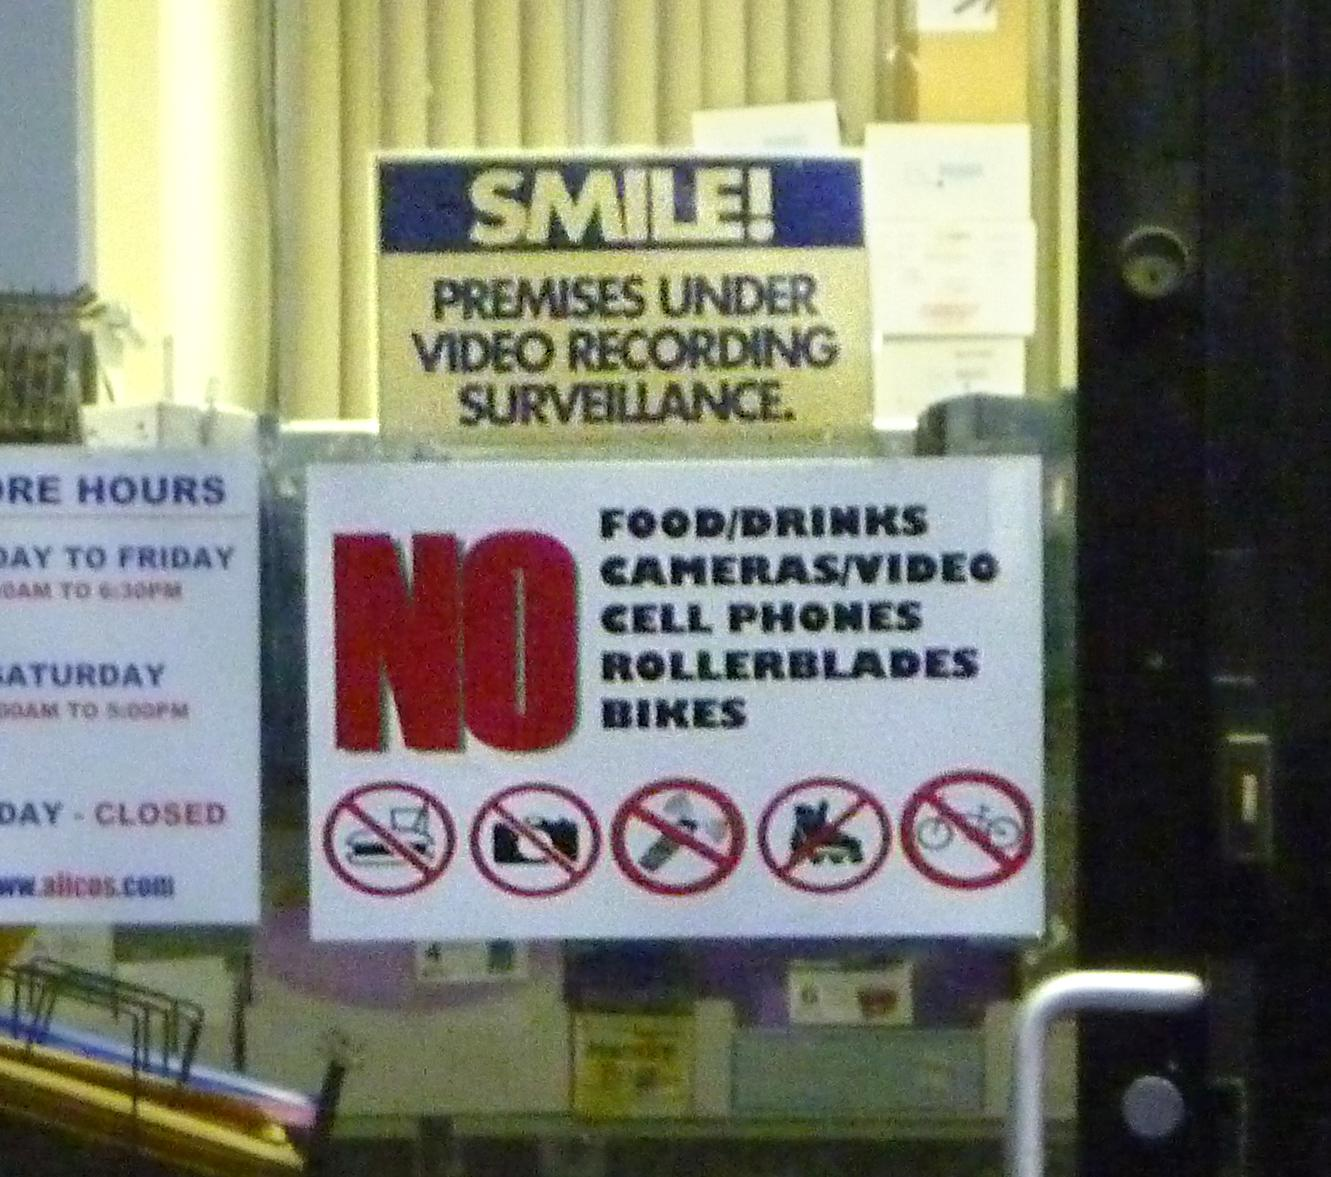
\includegraphics[height=2.83in]{ch5/figs/signoalicosproc2lowq.jpg}
  
\includegraphics[height=2.83in]{ch5/figs/advertisementQR_lowres.jpg}
    \caption{SMILE! 
             PREMISES UNDER VIDEO RECORDING SURVEILLANCE
             {\bf NO CAMERAS... NO CELL PHONES}
             Hypocrisy of Surveillance: Cameras simultaneously forbidden
             by policy, but
             required to read QR codes in many retail and business
             establishments.
            }
    \label{surveillancehypocrisy}
\end{figure}
In this way, {\em sur}veillance is the veillance of hypocrisy.

On that general theme, we've created a playful interactive art installation
as part of CONTACT PHOTOGRAPHY, the world's largest photography event.
CONTACT PHOTOGRAPHY is a photography festival that many different galleries,
museums, and other organizations partake in.
Our exhibit comprises a giant QR code on the front of a building
together with a ``NO CAMERAS'' icon/sign.

In a sense, the sign simultaneously says ``NO CAMERAS''
and ``CAMERAS REQUIRED''.
See Fig~\ref{building}.
\begin{figure*}[!t]
    \centering
    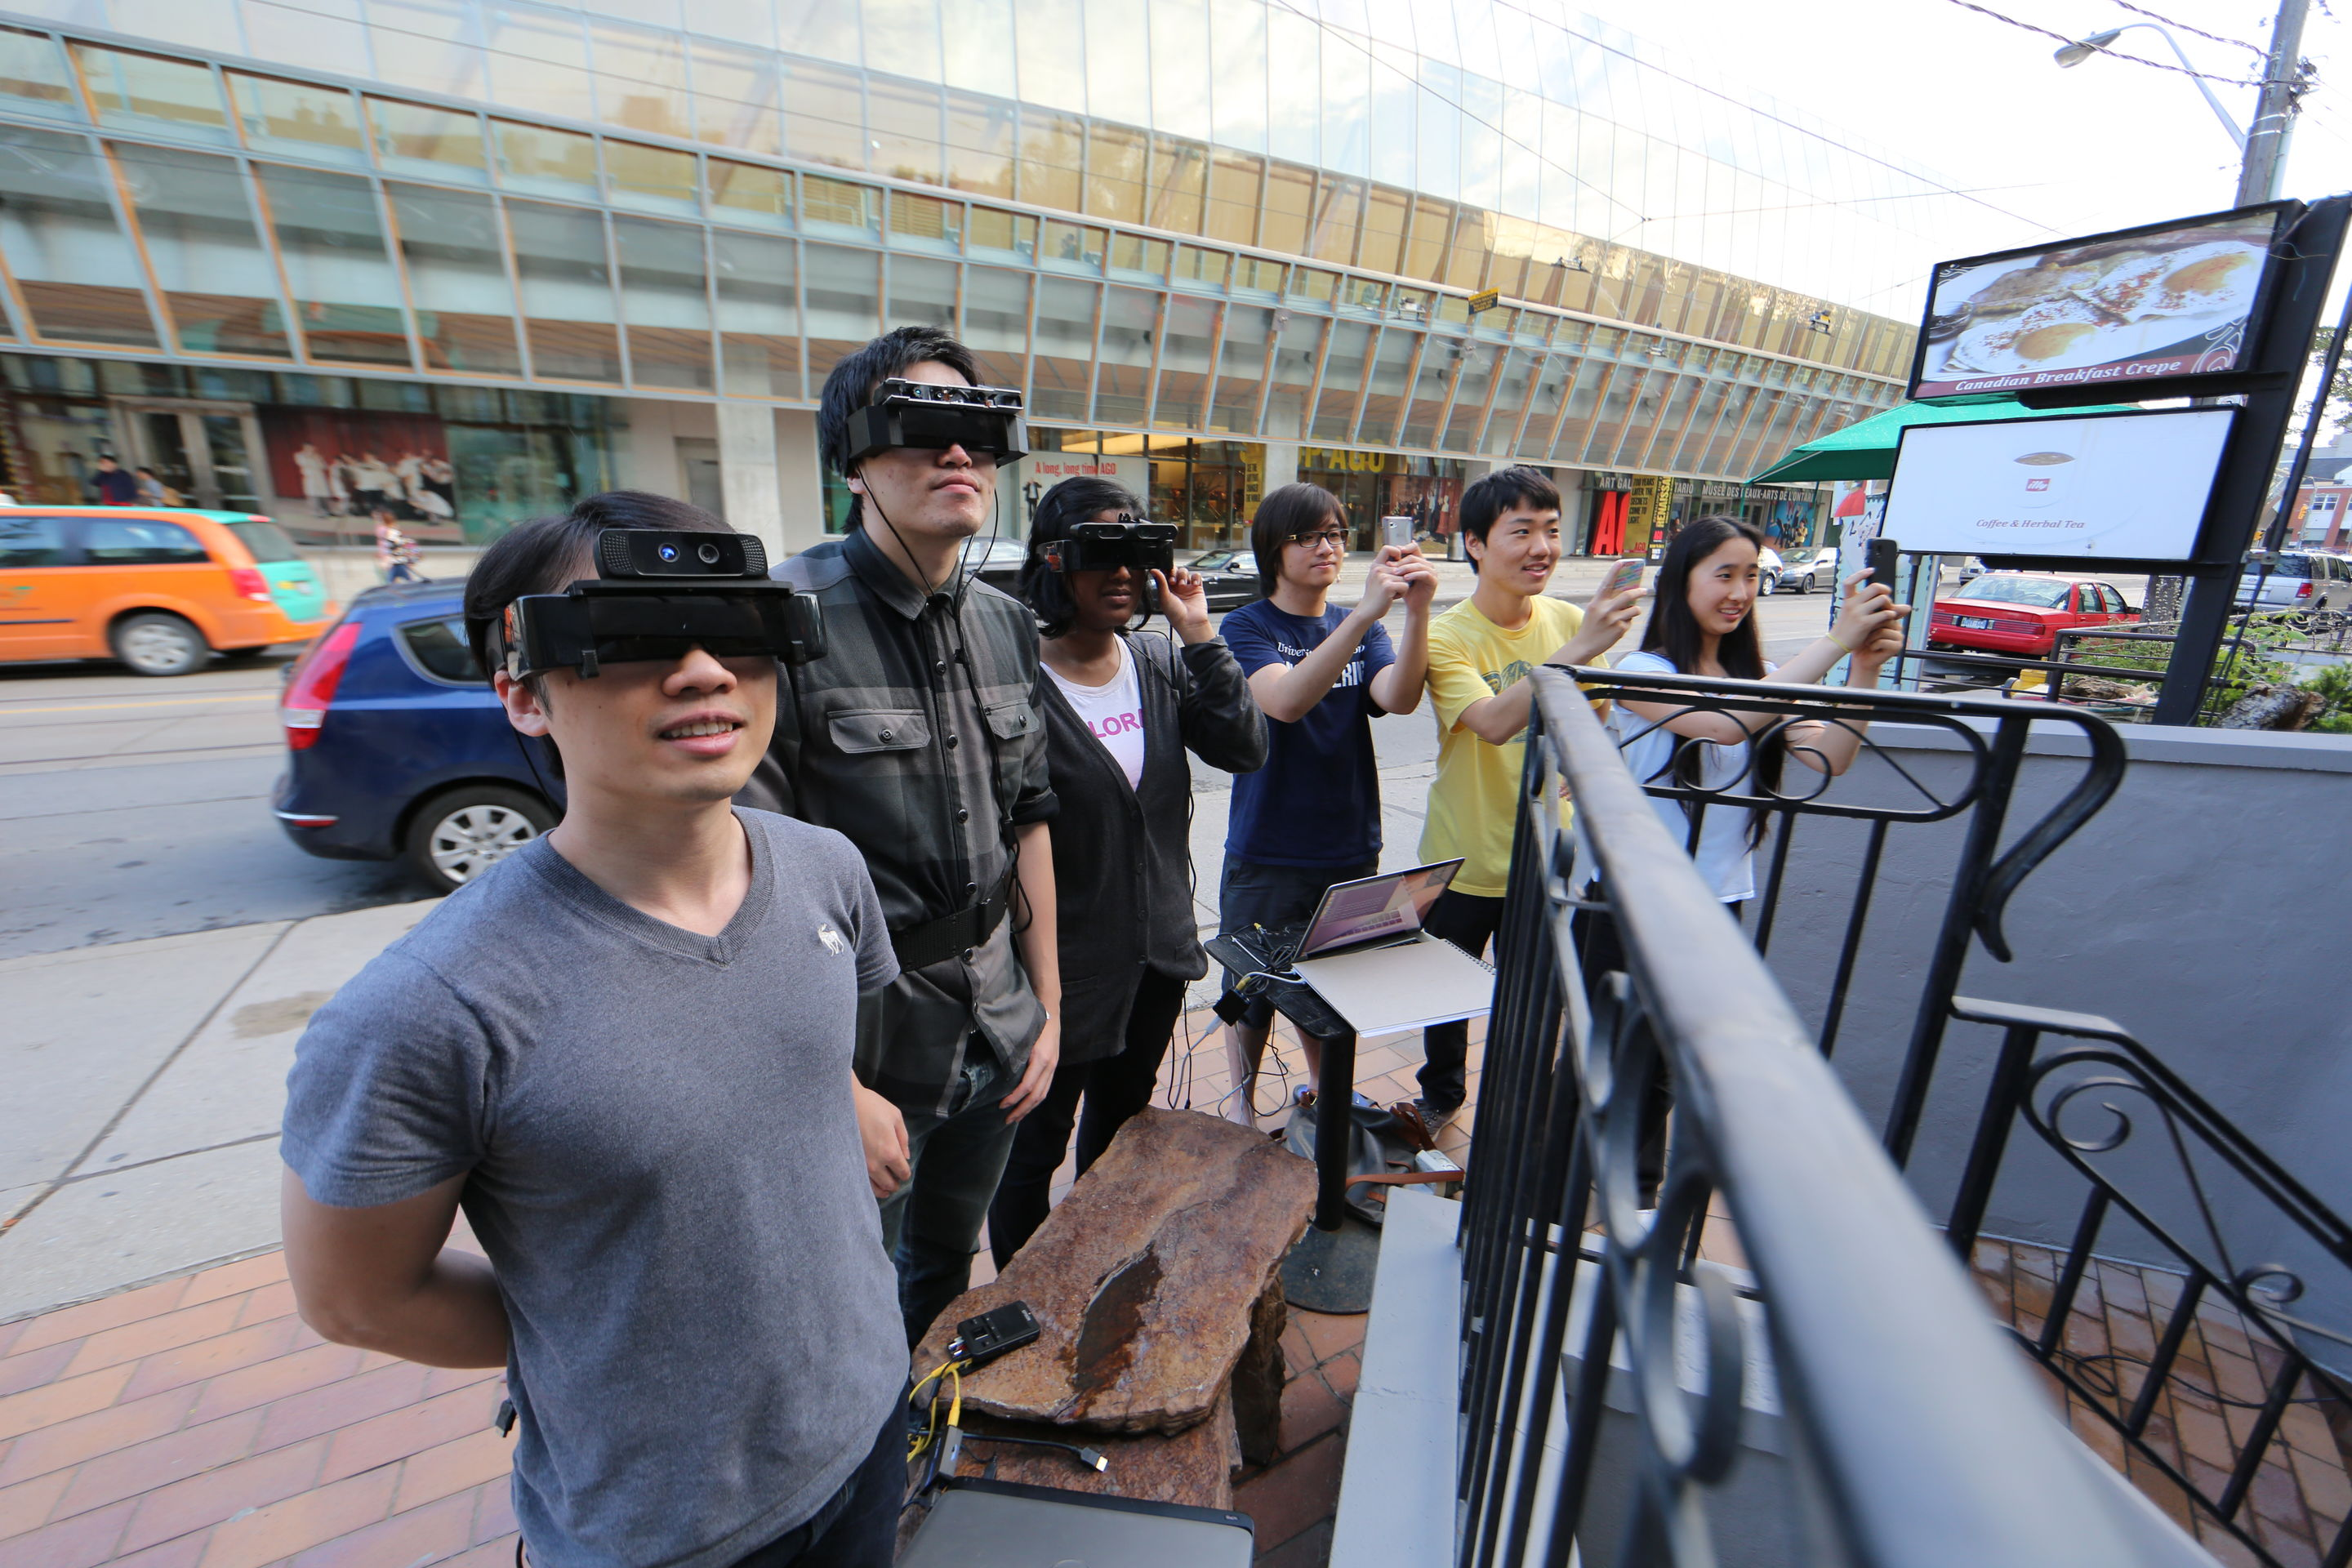
\includegraphics[height=2.5in]{ch5/figs/wearable/low_res/qr_3_eyeglass_IMG_2193.jpg}
    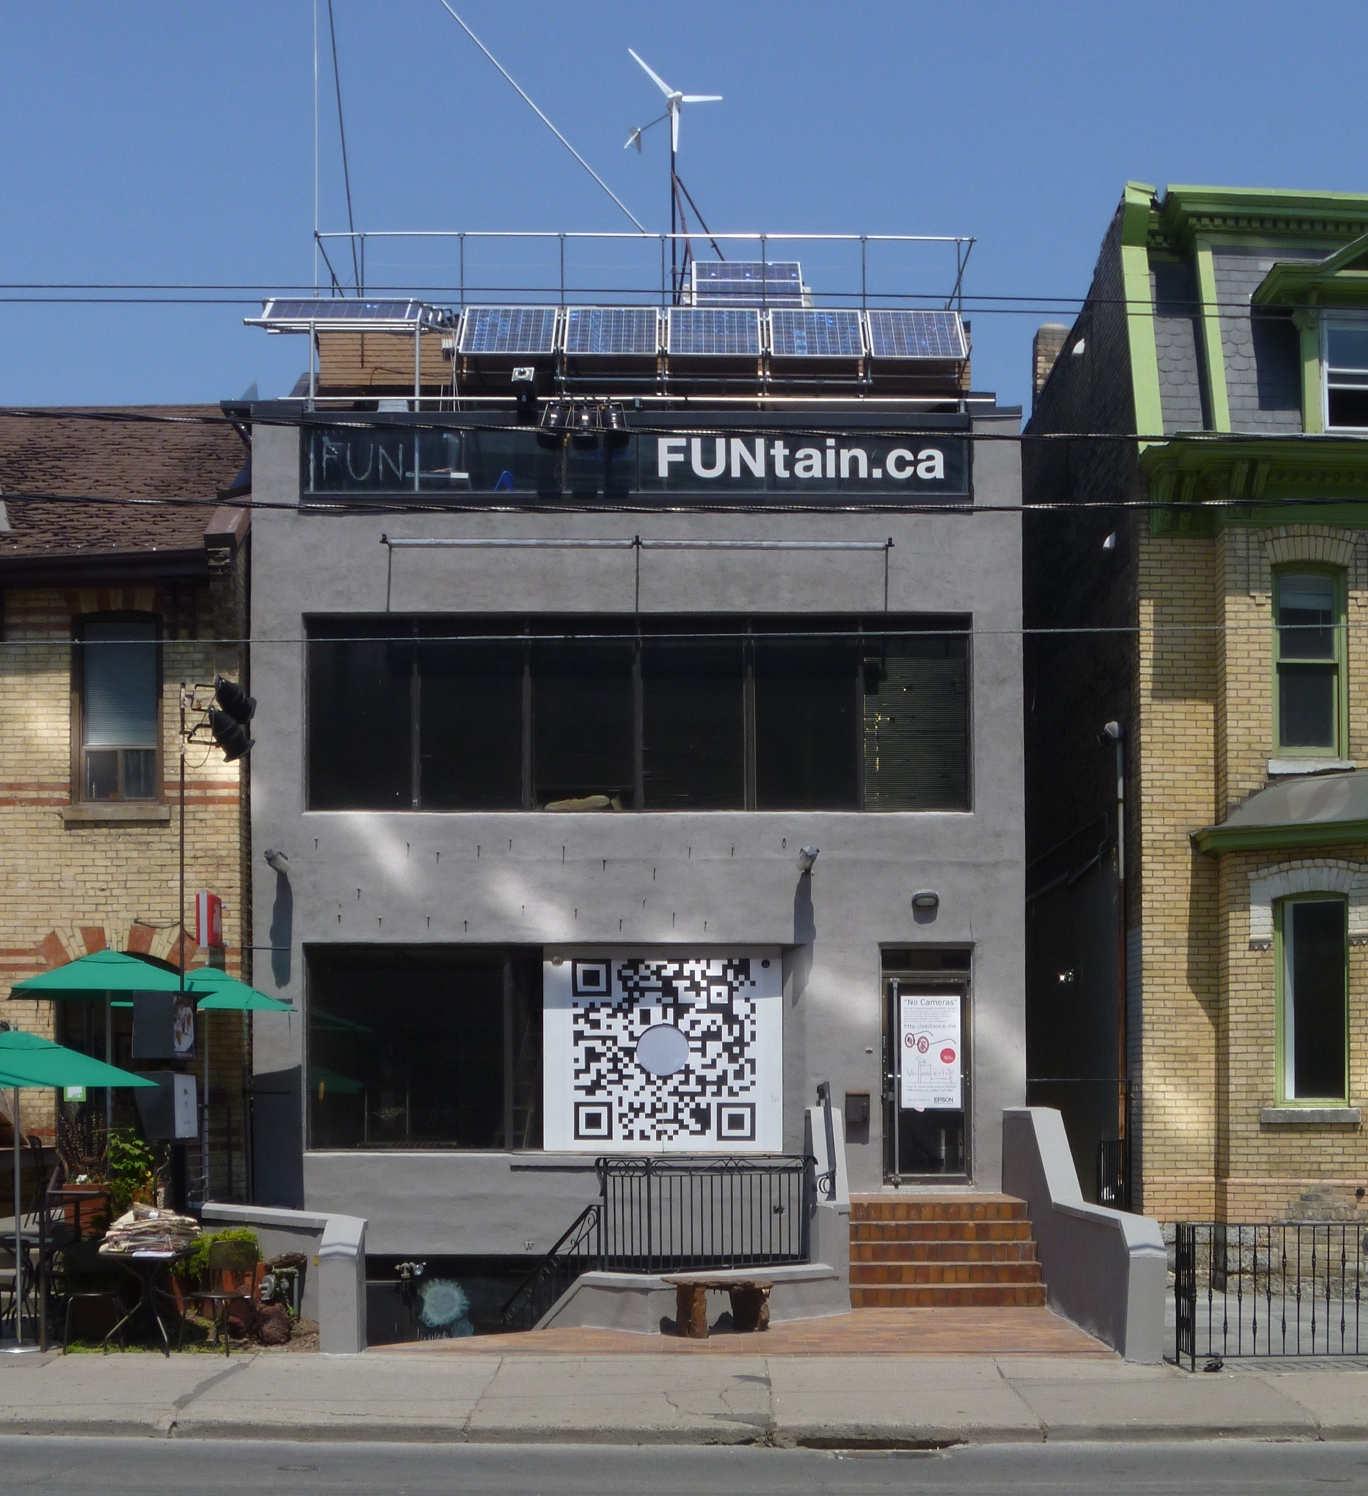
\includegraphics[height=2.5in]{ch5/figs/decon330dundasd2crop_lowres.jpg} \\
    \includegraphics[height=2.5in]{ch5/figs/QR-ISOVIEW_val_flipped.pdf}
    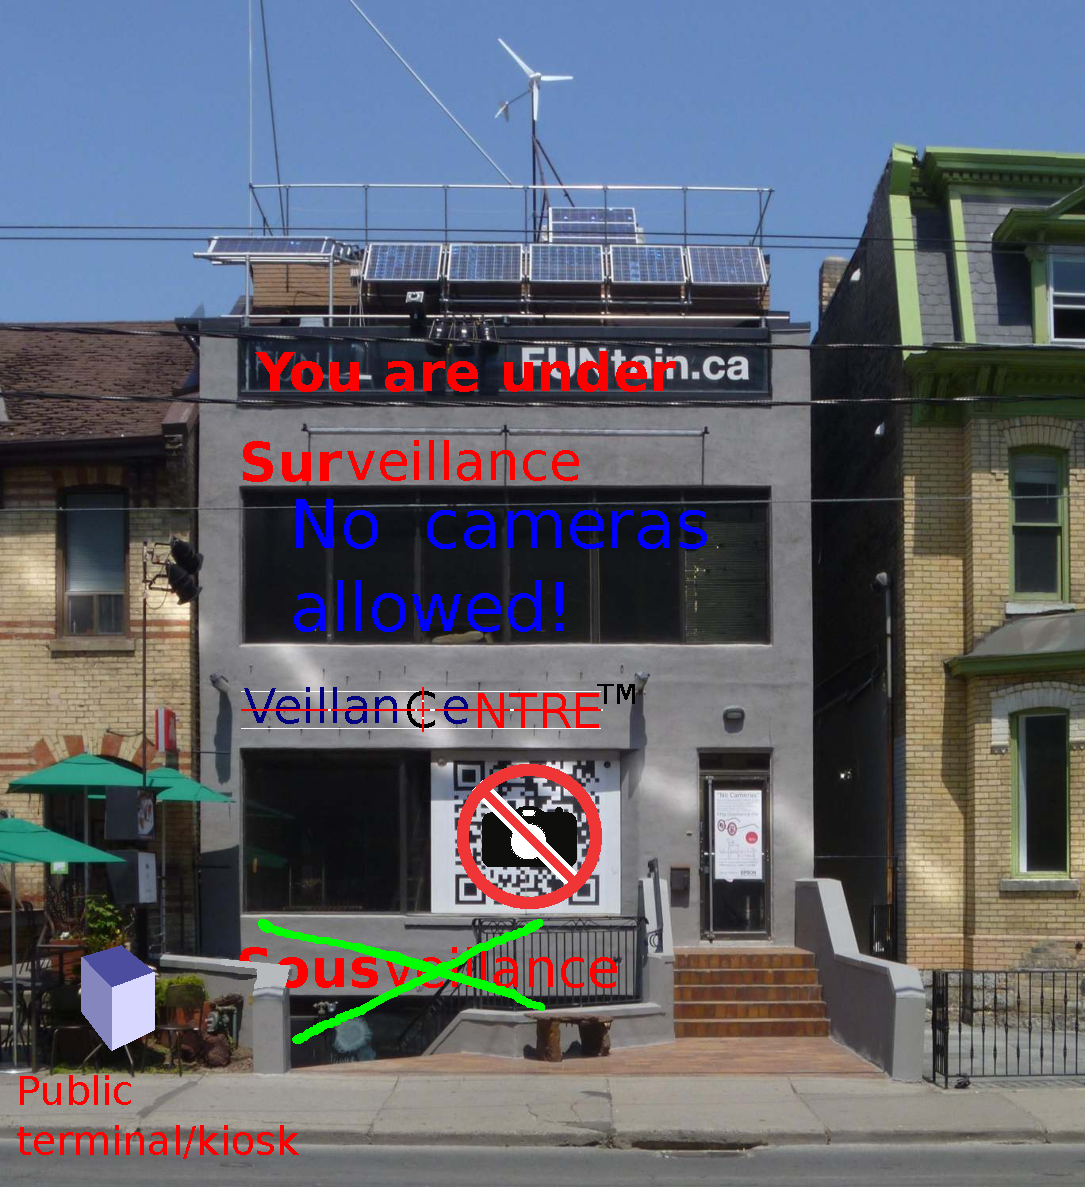
\includegraphics[height=2.5in]{ch5/figs/SurveillanceSousveillance330dundas4.pdf}
    \caption{Interactive QR code on a building.
             Users can interactive with the QR code
             signage by either capturing photos of
 the sign with a mobile phone or wearing FreeGlass. When an image of the sign
 is taken, the interactive QR code will automatically capture images of the
 audience/photographer with a flash (fire-back) and project the image onto the
 screen. With the wearable DEG (Digital Eye Glass), the QR images are
 scanned and information about the building is retrieved automatically.
 Such serendipitous recognition also includes gesture recognition to
 ``navigate'' the building interior from outside, and to ``navigate''
 through other information about a ``No Cameras!'' exhibit.
 The exhibit explores the notion of sousveillance and surveillance to
 allow photographers to understand the veillance-related issues such
 as the growing ``No photography'' mandate combined with increased surveillance
 in our society.
 This raises awareness of the hypocrisy that often accompanies
 surveillance in our daily life (i.e., the contradiction of having
 ``no photography''
 allowed while people are under the surveillance of the building's own
 camera/vision systems).
}
    \label{building}
\end{figure*}

The interactive mediated reality building Figure \ref{building} is a social
experiment and artistic in(ter)vention conducted by author S. Mann,
in collaboration with a team of researchers,
as a form of social inquiry into the use of sousveillance devices.
Photography and hand-held or wearable cameras are examples of sousveillance.
As common as such practices and devices are, there are still occasions when
photographers are harassed by security staff or police officials.
For example, persons with sousveillance devices are unwelcome in many
commercial establishments where numerous surveillance cameras are installed.
In this sense, surveillance is often the veillance of hypocrisy.
To understand this one-sided veillance, the interactive mediated reality
building was designed to take photos of any passing photographer as the
photographer scans the QR (Quick Response) code installed on the building.
As the photographer scans the QR code, he/she will see an augmented reality
sign indicating there is no photography allowed of the building.
Since the ``SIGNO'' (the round ``NO CAMERAS!'' sign in the center of the QR
code is not always visible), sometimes,
in order to scan the QR code and see this ``NO PHOTOGRAPHY'' sign,
the photographer must have already taken photos of the building. In either
case, the building will capture a photo of the photographer
and indicate that he/she is ``Wanted'' on suspicion of
violating the ``NO CAMERAS'' signs and/or policy displayed/purported
by the building. 
See infographic in Fig~\ref{infographic}.
\begin{figure*}
  \centering
  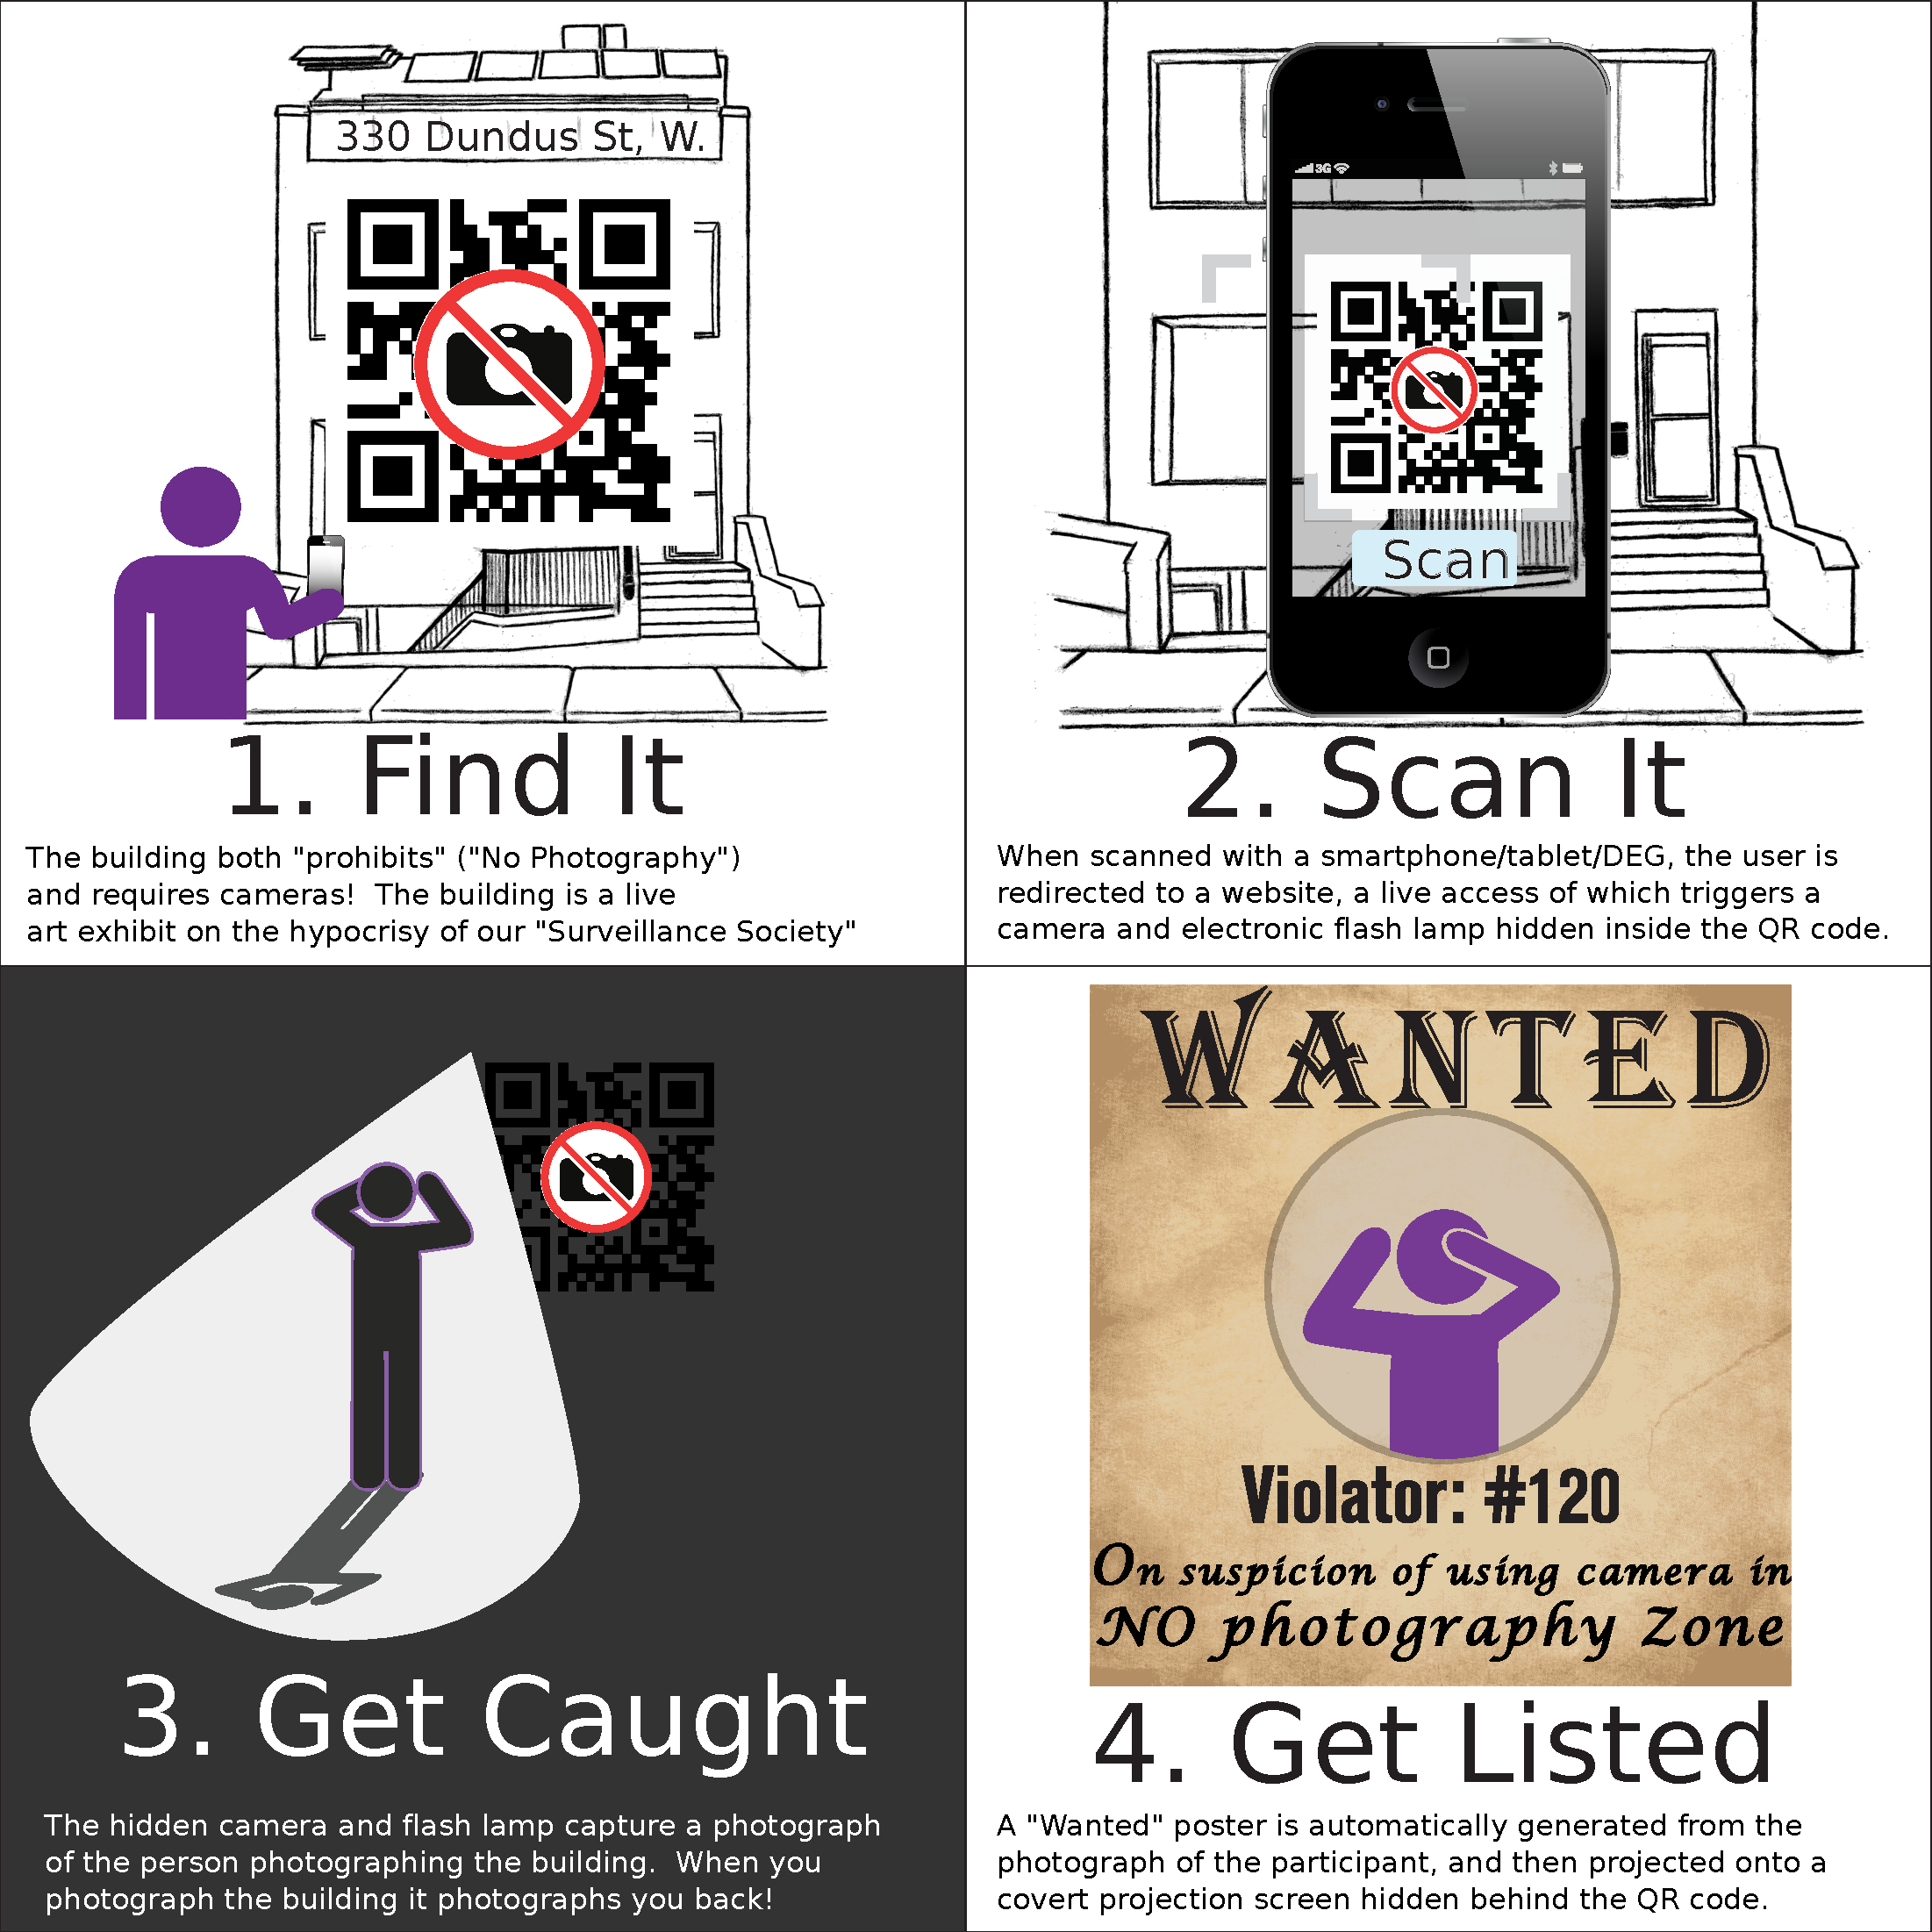
\includegraphics[width=6.0in]{ch5/figs/signo330infographics_small.pdf}
  \caption{If you photograph this building you get photographed and placed on
           a ``Wanted on suspicion of using camera in a no-photography zone''
           poster that is automatically generated and projected onto the face
           of the building for everyone in the area to see.  The
           ``Wanted'' posters are also visible online together with
           a ``Rogue Gallery'' of previous photography suspects.}
  \label{infographic}
\end{figure*}

In the past, people have implemented wearable gesture recognition algorithms based on a processing RGB frames fed from the sousveillance devices. To perform gesture recognition, these devices has to process every RGB frame in order to detect if there is any gesture command given by the user. As an example, the SixSense project uses a RGB camera to capture user's gesture command by detecting the color finger marker taped on the user's fingers. Another good example will be the telepointer \cite{mann2000telepointer}, which feeds RGB frames in order to provide a visual collaborative experience to the user. However, both projects requires constant polling on the RGB frame by the device, which has the potential to capture sensitive information of other surrounding people or environment. Thus, it has the potential to cause privacy intrusion. 

To avoid these privacy concerns caused by RGB based wearable gesture recognition system, our system uses an infrared (only) camera for gesture recognition.  Instead of polling for the RGB frames, we perform constant polling for the infrared frames. This approach not only achieves promising gesture recognition accuracy, but also avoids capturing sensitive information during its operation. 

%A wearable computer with gesture interface "frees" our hands of devices and enables us to interact with the world in a more "natural" way. However, like current hand-held devices, it still requires at least one of our hands to be free.%
Hand gesture is a form of expression. The presence of gesture helps to signal the person's action and its intention. A hand gesture controlled sousveillance device forces user's expression to both the camera of the system as well and the people around the user who are aware of such device. This deliberate act of expression as a command is a way to notify the crowd of user's action, which may reduce people's suspicion on the misuse of the sousveillance system. This is because the gesture commands have to be visible to the camera, in line of sight with the other subject matters that exist in the same view. Thus, the user has to be conscious of the consequence on his or her action to the surrounding being while commanding the sousveillance device. This may lead to a healthier veillance community for all users by reducing the anxiety caused by suspicion of privacy intrusion.

Aside from the use of camera technology, the hand gestures also pose some social implications. Because hand gestures is a form of expression and communication in our world, as each culture/country has its own spoken language, so too does each have its own set of hand gestures with their own meanings - there is no ``universal language" for gestures \cite{archer1997unspoken}. For example, the ``thumbs-up" gesture which carries a meaning synonymous to ``good-luck" in North America; in Iran, it carries a derogatory meaning - similar to the ``middle-finger" in North American culture. Thus, if a wearable system is designed with a fixed set of gestures, it is possible that these gestures have different meanings in different cultures - some of which may even be offensive. Therefore, having a fixed set of gestures can affect the global acceptance of a gesture-based wearable computer unless the gestures and their meanings become universally accepted. For example, the ``upper-left" and ``lower-right" gesture together (as shown in Figure \ref{bounding}), can be a global gesture for taking a picture in the selected area of view. Another solution is to design the gesture system to account for the cultural differences, that is, the gesture system is localized by country. However, whenever a user travels to a different country, the user will have to relearn the gestures required to interact with their wearable computer, and this can be inconvenient for the user.

\section{Future Work}
In further development of the FreeGlass system, we are experimenting and
expanding on our current base to incorporate more gestures to our system
and create more ways for the user(s) to interact with their environment in
first person perspective. For example, we are currently developing a sport
aid system that helps a billiards player improve their skills. We are
incorporating new gestures in this application to enable a user to segment
the relevant ball and find the optimal path to hit the ball into the pocket.
We also developed an underwater version of FreeGlass to assist hydraulists
in playing and learning how to play hydraulophone, as well as for use of
hydraulophone in rehabilitation exercises and underwater health improvement
exercises, gaming, and the like.
Additionally, we have developed various prototypes based on different 3D
sensing technologies, e.g., time-of-flight and structured-light.

More advanced 3D sensors, namely a hybrid approach which takes advantage
of the short range SoftKinetic's time-of-flight 3D sensors and
the PrimeSense's structural light IR laser 3D sensors, will provide a
more robust and rich user experience. The miniaturization of the FreeGlass
system with these sensor components also plays an important role in having
such a device available to enable further research
to be explored on a larger scale.

\section{Conclusion}
We have proposed FreeGlass, a 3D self-gesture-sensing wearable computer system utilizing a 3D camera.
We process information from the range camera, in real time, to recognize
hand gestures. Once we get the user input through the range camera, we
display the interaction, such as the corresponding action due to a gesture,
back to the user via the Epson Moverio BT-100 display. We trained a
neural network learning algorithm to learn various gestures
to demonstrate a prototype of our gesture interface
and achieved 99.8\% training accuracy, 96.8\% testing accuracy.
We are able to run this recognition system at interactive frame rate
(25-30fps) on an ODROID-X2 (a miniature portable or ``mobile'' computer).

FreeGlass is a low-cost easy-to-implement wearable computer system that
provides uses with an ability to tinker and experiment with various
possibilities.  We also explored issues of Technology \& Society,
such as by way of an interactive ``Hypocrisy Building'' that photographs
people who photograph the building, thus exploring issues of
veillance (surveillance versus sousveillance).


